The purpose of this chapter is to provide quantitative upper and lower-bound estimates on the expected electron flux due to LEP, as a function of location and time of year. We expand on the raytracing and interpolation method described in chapter \ref{chapter:power}, by incorporating a resonant-particle scattering code. We compute global electron fluxes in a similar manner as in Chapter \ref{chapter:power}, using an array of precomputed stencils, which we scale and shift according to GLD360 data. Finally, we can examine the relative timescales on which LEP could deplete a populated magnetic field line, in the absence of any other loss processes.

\section{Resonant Interactions}
As discussed in section \ref{section:wpi}, the interaction between waves and trapped particles has a cumulative effect only when certain resonant conditions are met. The condition for resonance is given by:
\begin{equation}
\frac{d\eta}{dt} = m \omega_c/\gamma - \omega - k_z v_z = 0
\label{eqn:resonance_cond}
\end{equation} 
where m is the resonance order number, $\gamma = (1 - v^2/c^2)^{-1/2}$ is the Lorentz relativistic correction factor, $\omega_c$ is the local cyclotron frequency, and $k_z$ and $v_z$ are the parallel components of the wavenormal vector and particle velocity with respect to the background magnetic field. The angle between the wave magnetic field vector and $v_\perp$ is given by $\eta$.

We assume any perturbation in pitch angle is small, and can therefore only concern ourselves with particles very near the edge of the loss cone. We can therefore relate the total velocity $v$ and the parallel velocity $v_z$ via $v^2 = v_z^2/\cos^2\alpha_{lc}$ \citep{Lauben2001, Bortnik2006}.

Plugging in the above terms for $\gamma$ and $v_z$ gives us the following closed-form expression for the resonant particle velocity for an incident wave:
\begin{eqnarray}
v_z^{res} & = & \bigfrac{\pm \sqrt{\omega^2 k_z^2 + \left[ (m \omega_c)^2 - \omega^2 \right] \left[k_z^2 + (\frac{m \omega_c}{c \cos \alpha_{lc}})^2\right]} - \omega k_z}{k_z^2 + (\frac{m \omega_c}{c \cos \alpha_{lc}})^2} \unit{m/sec}
\label{eqn:vzres}
\end{eqnarray}

The resonant kinetic energy can then be related by:
\begin{eqnarray}
v_z^{res} = \|v_{res}\|\cos\alpha_{lc}  \unit{m/sec}\\ 
E_{res} = \frac{E_{0}}{\sqrt{1 - v_{res}^2/c^2}} - 1 \unit{J}
\end{eqnarray}

\noindent where $E_{0}$ is the particle rest energy ($\approx$ 511 keV for an electron).

Equation \eqref{eqn:vzres} is a function of the incident wave, which is dependent on the wavenormal angle and the background plasma through $k_z$. We can illustrate broad trends by plotting resonant frequency vs kinetic energy along the geomagnetic equator, for normal incidence ($k = k_z$). Figure \ref{fig:vzres_vs_modes} shows the resonant frequency for a range of L-shells, for m = $\{0,1,2\}$. Somewhat counterintuitively, lower-energy particles resonate with higher-frequency waves.

L-shell dependence is due both to the background electron density through $k_z$, and the background magnetic field through $\omega_c$. Particles at higher L-shells resonate with lower-frequency waves.

\begin{figure}[h]
\begin{center}
%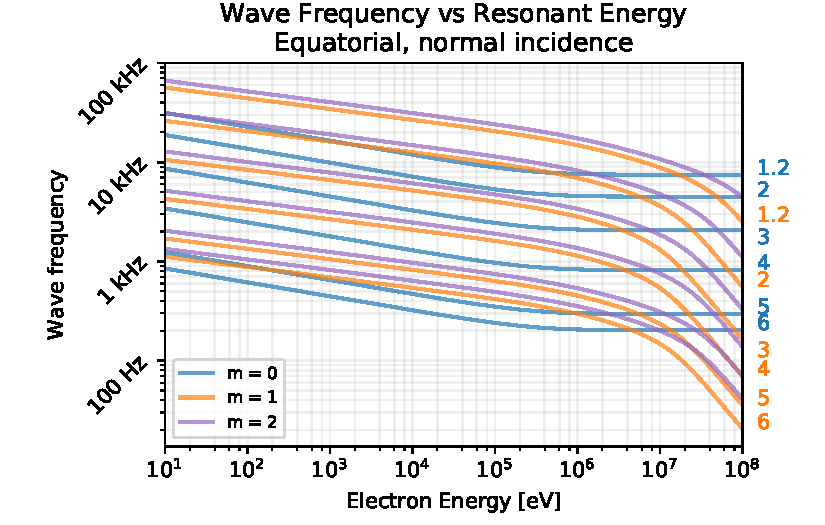
\includegraphics{figures/wave_frequency_vs_energy_vs_mode.pdf}
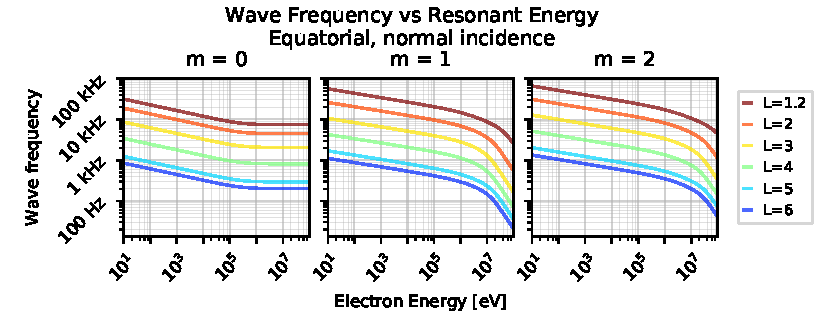
\includegraphics{figures/wave_frequency_vs_energy_vs_mode_3up.pdf}

\caption[Resonant frequency vs particle energy for resonant modes 0, 1, and 2]{Resonant wave frequency vs trapped electron kinetic energy, for resonant modes m = 0, 1, and 2. Shown here for resonances along the geomagnetic equator, with normal incidence. The background plasma is modeled for \kp{}=0 using the Simplified GCPM model in section \ref{section:plasmasphere_models}.}
\label{fig:vzres_vs_modes}
\end{center}
\end{figure}

At lower energies, the resonant modes are integer multiples of each other; however as the particles become increasingly relativistic, the modes deviate substantially. Most significantly, when setting $m=0$, the relativistic term vanishes completely, and the resonant frequency asymptotes.

\subsection{Calculating pitch-angle scattering vs time}

Calculating pitch-angle perturbations incurs additional complexity as compared to the energy density estimate in Section \ref{chapter:power}. Pitch-angle scattering is dependent on wave amplitude and frequency, as well as incident wavenormal angle $\theta$ and gyrophase $\eta$. Additionally, the formulation for pitch-angle scattering requires wave amplitudes with units of (Poynting) energy flux, $\mathrm{1/m^2/s}$, rather than volumetric densities, $\mathrm{1/m^3}$.

The fundamental pitch-angle scattering equation is given in equation \eqref{eqn:bell_dadt}, and reproduced below:
\begin{equation}
\frac{d\alpha}{dt} = \underbrace{\frac{m_e \omega_{\tau m}^2}{k_z p_\perp} \bigg( 1 + \frac{\cos^2\alpha}{m\,\omega_c / \omega - 1}\bigg)}_{T_1}\underbrace{\sin \eta}_{T_2} + \underbrace{\frac{1}{m_e \gamma}\frac{p_\perp}{2 \omega_c}\frac{\partial \omega_c}{\partial z}}_{T_3} \unit{rad/sec}
\label{eqn:bell_dadt_with_labels}
\end{equation}

Terms $T_1$ and $T_3$ are slowly-varying, and can be treated as pseudo-constant at a fixed position in space. Term $T_2$ in \eqref{eqn:bell_dadt_with_labels} is the resonant component. Outside of resonance this term oscillates between $\pm 1$. At resonance, however, this term remains constant, allowing coherent changes to accumulate over the interaction period. Resonance implies only that $d\eta/dt = 0$, and provides no information on the value of $\eta$. We assume $\eta$ is uniformly distributed, in which case the perturbation in pitch angle $d\alpha/dt$ will be sinusoidally distributed, symmetrically about zero \citep{Inan1977}. Since we are concerned only with the distribution of particles which are perturbed into the loss cone ($d\alpha/dt < 0$), we can then track the RMS-average pitch angle change $\Delta \alpha_{RMS}$, and calculate the precipitated fraction using the uniform distribution (see section \ref{section:flux_from_pitch_angle}).
Figure \ref{fig:test_particle_sims} shows an example of a test-particle simulation, in which a set of particles with different initial $\eta$ values are subjected to the same perturbing wave.

\begin{figure}[t]
\begin{center}
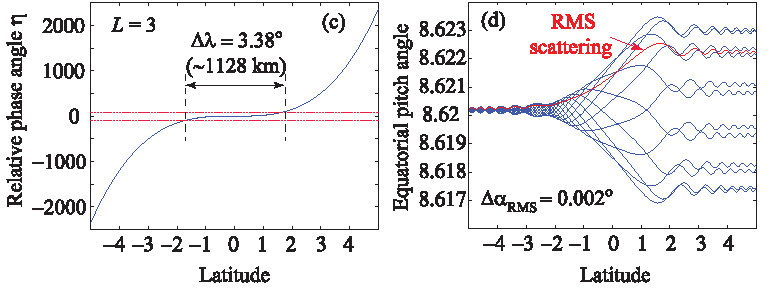
\includegraphics{figures/Bortnik_RMS_scattering.pdf}
\caption[RMS pitch angle scattering from a test particle simulation]{Comparison of RMS and peak deflection in pitch angle from a test particle simulation. On the left is shown the relative gyrophase angle, which must be constant in order for changes to accumulate. On the right is the pitch angle of an array of particles, each with a different initial gyrophase. After the interaction has occurred, the perturbed pitch angles are symmetric about the initial pitch angle. The red curve shows the RMS change. Figure taken from \cite{Bortnik2006}, Figure 7.}
\label{fig:test_particle_sims}
\end{center}
\end{figure}

From here, we follow the numerical solution method from \cite{Bortnik2005, Bortnik2006}. 

A key assumption in our scattering calculation is that the interactions on a single particle from each discrete frequency are independent from one another. Furthermore, we discretize each fieldline into 1$^\circ$ segments, and assume the scattering within each segment is independent from each other. While neither of these assumptions are exactly true, together they provide a critical and substantial reduction in complexity: we no longer have to track the action of the entire set of waves on a discrete set of particles (as in a test particle simulation such as \cite{Chang1985}), but rather can track the stochastic pitch-angle change on a distribution of particles. Additionally, by assuming incoherent scattering across frequencies, the problem becomes much more well-suited to a parallel processing solution, as we can spread computation for each frequency across an array of nodes.\footnote{The coherent-incoherent assumption is based on test particle simulations such as \cite{Chang1985} and \cite{Ristic1993}; however a modernized test-particle (time domain) validation of the approach would be an excellent opportunity for future work!}

Thus, for each set of guide rays $F$, using the interpolation scheme from section \ref{chapter:power}, we can calculate $\Delta \alpha_{RMS}$ as a function of magnetic fieldline, particle energy, and time; the effective change in pitch angle is then determined by summing over the set in quadrature: 
\begin{equation}
\Delta \alpha(E, \vec{x}, t) = \frac{1}{2}\sqrt{\sum_{F} \Delta \alpha_{RMS}^2(E, \vec{x},t, F)}.
\end{equation}

The decision to calculate RMS pitch-angle scattering versus a full test-particle approach is the fundamental difference between \cite{Lauben1998} and \cite{Bortnik2005}, the two most-closely related works to ours. \citeauthor{Bortnik2005} uses the above method, while \citeauthor{Lauben1998} infers expected distributions from a set of test particles. 

As noted by \cite{Lauben1998, Lauben2001}, a subset of particles, when subjected to ideal conditions, can ``ride'' a perturbing wavefront across several degrees in latitude, and experience sustained, coherent perturbation. These particles would then precipitate very deeply into the ionosphere, which may account for the lowest-altitude ionization as measured using VLF sub-ionosphere sensing. However these particles represent only a small fraction of the precipitating electrons, the bulk of which experience a random walk through the set of perturbing waves, and are well-modeled by the stochastic RMS formulation of \citeauthor{Bortnik2005}.

\citeauthor{Bortnik2005} makes several approximations which allow for quick numerical integration of \eqref{eqn:bell_dadt_with_labels}, the details of which are beyond the scope of this dissertation. For a concise description of the methodology, see \cite{Bortnik2006}. Table \ref{alg:RMS_change} shows the algorithm in pseudocode. Using the assumptions of incoherence described above, we can independently calculate squared pitch-angle change for every enumerated combination of: a) guide ray sets $F$, b) latitudes along an output fieldline $\lambda$, c) time steps $t$, d) resonant modes $m$, and e) resonant particle energies $E$. 

\begin{algorithm}[t]
\caption{RMS change in pitch angle}\label{alg:RMS_change}
\begin{algorithmic}[1]
\ForAll{output field lines}
	\State{d$\alpha$\_N $\gets$ Zeros(E, t)}\Comment{Pitch angle change at northern hemisphere}
	\State{d$\alpha$\_S $\gets$ Zeros(E, t)}\Comment{Pitch angle change at southern hemisphere}
	\ForAll{sets of guide rays}
		\State{Scale input energy according to input flash location and frequency}
		\ForAll{latitudes along field line $\lambda$}
			\ForAll{time steps $t$}
				\ForAll{resonant modes $m$}
					\State{Calculate $V_{res}$, $E_{res}$}
					\ForAll{grid energies within resonance band $E$}
						\State{$\Delta \alpha_{cur} \gets \int_{t1}^{t2} \frac{d\alpha}{dt}$}
						\State{tN $\gets$ t + $\tau_{f,N}$} \Comment{flight time to northern ionosphere}
						\State{tS $\gets$ t + $\tau_{f,S}$} \Comment{flight time to southern ionosphere}
						\State{d$\alpha$\_N[E, tN] += $(\Delta \alpha_{cur})^2$}
						\State{d$\alpha$\_S[E, tS] += $(\Delta \alpha_{cur})^2$}
					\EndFor
				\EndFor
			\EndFor
		\EndFor
	\EndFor
	\State{d$\alpha$\_N $\gets \sqrt{\mathrm{d}\alpha\_\mathrm{N}}$}
	\State{d$\alpha$\_S $\gets \sqrt{\mathrm{d}\alpha\_\mathrm{S}}$}
\EndFor
\end{algorithmic}
\end{algorithm}


To account for variation in precipitation time, we record the perturbation in pitch angle at the time in which a perturbed particle would precipitate into the atmosphere. This time is dependent on both particle energy and the latitude along the field line where the perturbation occurred, and may be asymmetric between the northern and southern hemispheres.

We compute the time of flight from the interaction latitude $\lambda$ to the ionosphere by assuming a perturbed particle continues along a fixed fieldline, by numerically evaluating the expression from \cite{Walt1994}, equation 4.25:

\begin{equation}
\tau_f =  \frac{1}{v} \int_{s_1}^{s_2} \bigg(1 - \frac{B(s)}{B_{eq}}\sin^2\alpha_{eq}\bigg)^{-1/2} \mathrm{d}s
\label{eqn:bounce_time}
\end{equation}

\subsection{Example energy-time spectra}
Figure \ref{fig:dA_spectra} shows a typical pitch-angle scattering matrix, as a function of electron energy and time delay from a lightning flash at $35^\circ$ latitude, with $I_0=-10$kA. A similar scattering matrix must be computed for every point in the output space (L-shell and longitude offset).

\begin{figure}[h]
\begin{center}
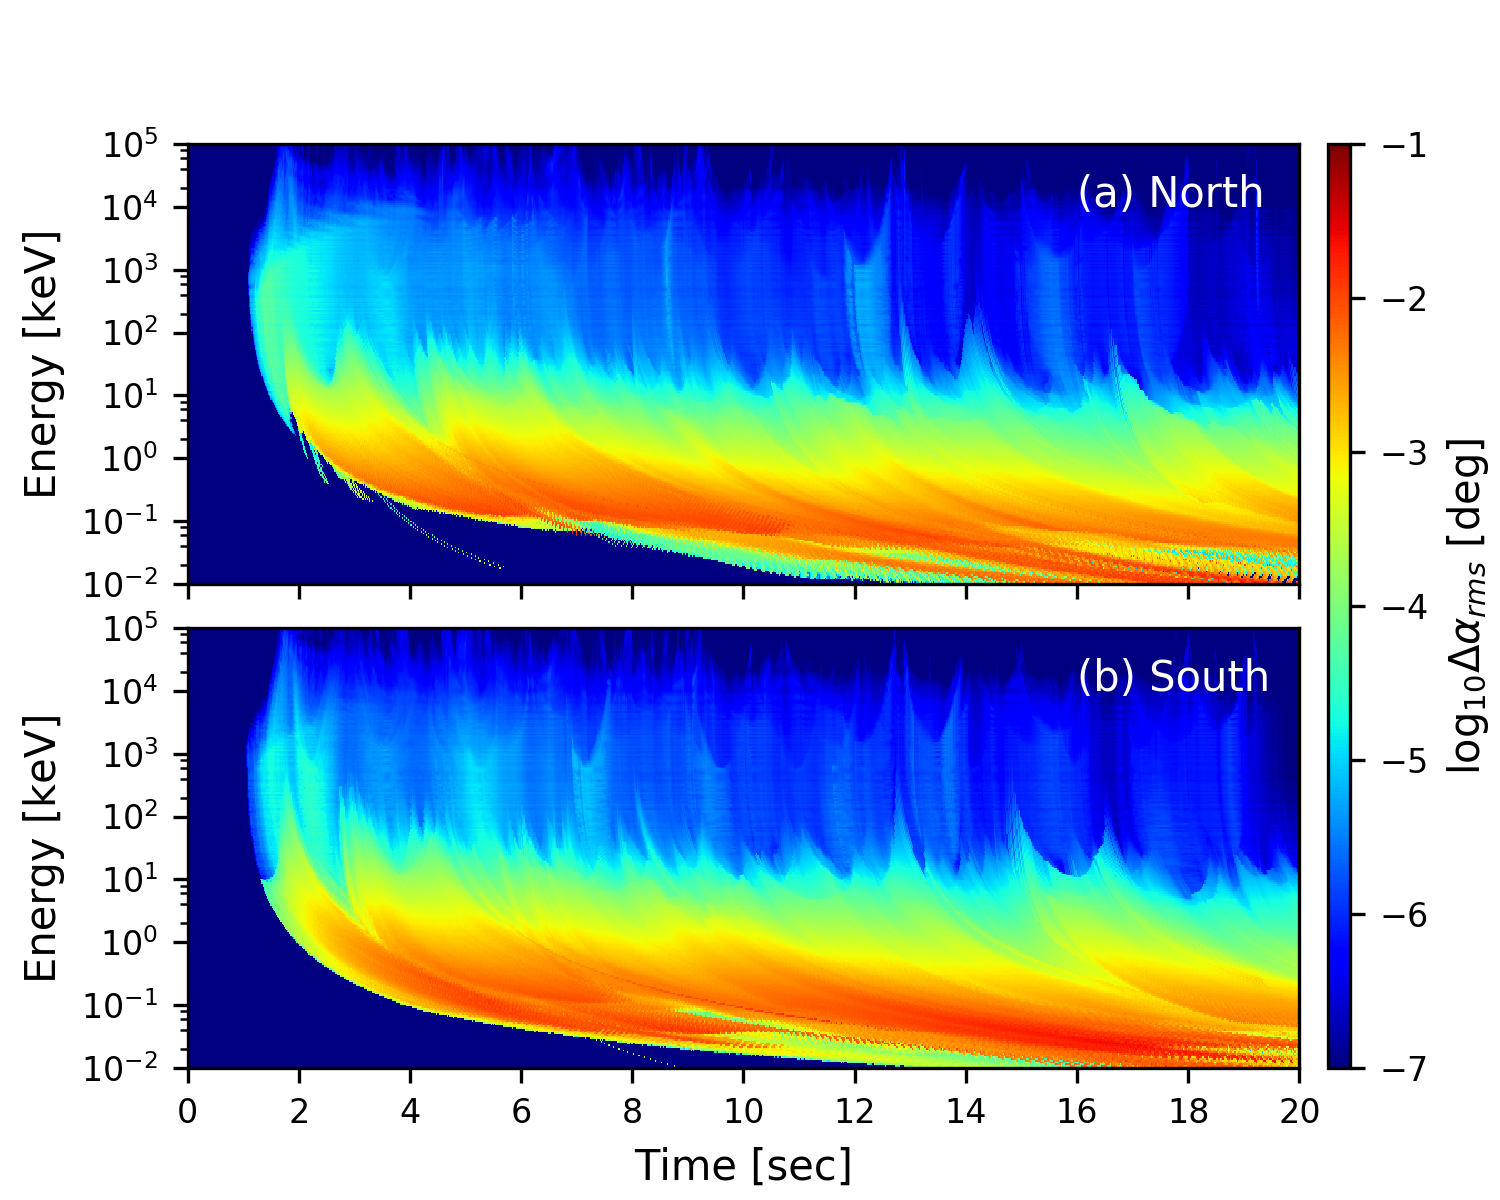
\includegraphics{figures/dA_E-t_spectra.png}
\caption[Pitch angle scattering matrix for a flash at 35$^\circ$ latitude and L=3]{Pitch angle scattering matrix along a fieldine with L=3, for a 10 kA flash at 35$^\circ$ latitude, through a nightside ionosphere at \kp{}=0. Scattering is centered directly over the input flash longitude, within a width of $\pm0.25^\circ.$}
\label{fig:dA_spectra}
\end{center}
\end{figure}

Several key features are apparent: First, the descending curve shape is due to the time delay from the interaction region to the precipitation altitude, with slower moving electrons taking longer to reach the ionosphere. Two banded structures are visible with respect to energy: the dominant band, below $E \sim 10$ keV, is due to the 0-order resonance mode. The upper band with energies above $E  \sim 100$ keV, is due largely to the $\pm$ 1 resonance modes. Scattering efficiency decreases with increasing resonance order, due to the presence of order number $m$ in the denominator of equation \eqref{eqn:bell_dadt_with_labels}, term T1. While some asymmetry exists between the northern and southern hemispheres, the magnitude remains similar due to the numerous bounces of the incident waves, and because the higher-order modes resonate with particles traveling in either direction.

Perturbations in pitch angle due to LEP are generally small; well below $0.1^\circ$. However, due to the exponentially-increasing density of the ionosphere below our threshold height of 100 km, and thus the very small change in reflection altitude required, small changes in pitch angle can greatly increase an electron's likelihood of precipitating. Figure \ref{fig:pitch_angle_vs_altitude}(a) shows the perturbed reflection altitudes versus L-shell, for an array of $\Delta \alpha$ values. Figure \ref{fig:pitch_angle_vs_altitude}(b) shows the minimum perturbation value required in order for a particle to reflect at a given altitude.

\begin{figure}[t]
\begin{center}
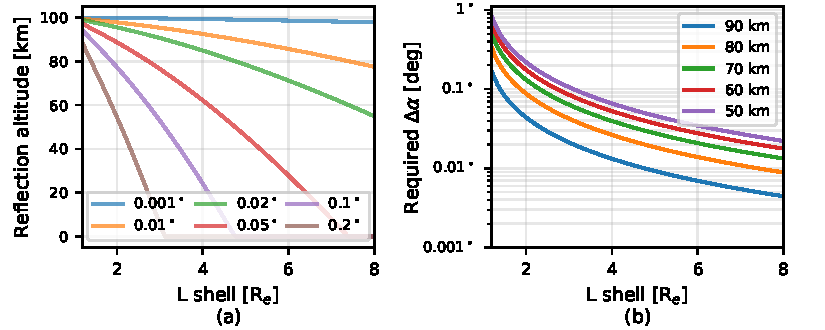
\includegraphics{figures/pitch_angle_vs_depth.pdf}
\caption[Reflection altitudes vs L-shell for a set of pitch angle perturbations]{(a) Reflection altitude vs L-shell for a particle, for an array of equatorial pitch-angle perturbations. (b) The minimum perturbation required to drive a particle with pitch angle $\alpha = \alpha_{lc}$ to a fixed reflection altitude, as a function of L-shell, for an array of target altitudes.}
\label{fig:pitch_angle_vs_altitude}
\end{center}
\end{figure}


\section{Calculating flux from pitch-angle perturbations}
\label{section:flux_from_pitch_angle}
We have now computed the RMS change in pitch angle along a single field line, as a function of electron energy and time, for a single lightning flash. Next we must convert our scattering matrices (Figure \ref{fig:dA_spectra}) into electron fluxes (or energy fluxes). Again, we follow the method used by \cite{Bortnik2005} (section 5.1.3).

Along each target fieldline, we use our calculated pitch angle changes $\Delta \alpha(E,t)$ to perturb a collection of electrons with an assumed distribution in pitch angle. Perturbation is accomplished by convolving an assumed distribution of particles $G(E,t,\alpha)$ with the perturbing function $\Delta \alpha(E,t)$ for each energy and time bin. The resulting particle flux is the number of electrons within the loss cone ($\alpha < \alpha_{lc}$) after perturbation. We assume that scattering is independent with respect to both the time and energy axes, and can thus be evaluated independently for each $E-t$ bin. Solving the convolution analytically greatly improves computational efficiency.

We use the solution from \cite{Bortnik2005} for a ``ramp'' distribution in pitch angle, which can be applied to any general pitch angle distribution by computing a series approximation about $\alpha = \alpha_{lc}$.

\begin{equation}
% Bortnik figure 5.8, equation d.  
% Maybe you should include a figure here too?
\end{equation}


\begin{figure}[t]
\begin{center}
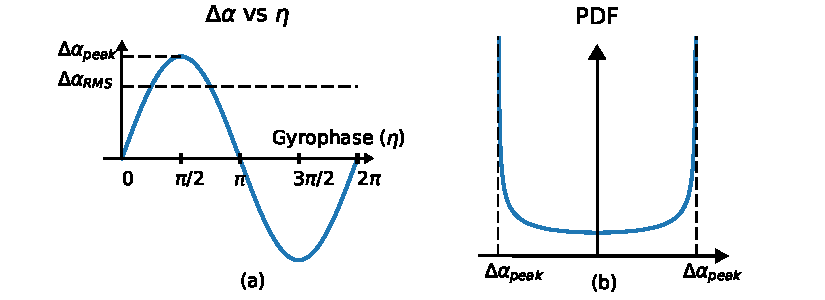
\includegraphics{figures/da_dist_and_pdf.pdf}
\caption[Pitch angle perturbation vs gyrophase, and corresponding PDF]{(a) Pitch angle perturbation vs particle gyrophase, with $\Delta \alpha_{rms}$ marked, and (b) The corresponding probability density function (PDF, equation \eqref{eqn:pdf}). Modified from \cite{Bortnik2005}, Figure 5.8.}
\label{fig:da_vs_eta_and_pdf}
\end{center}
\end{figure}

\begin{figure}[h]
\begin{center}
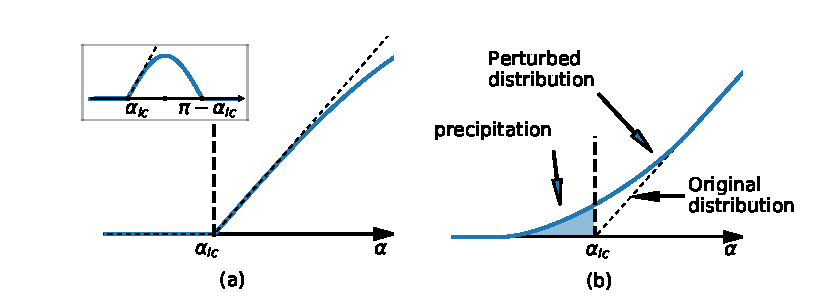
\includegraphics{figures/da_dist_and_perturbation.pdf}
\caption[Perturbed pitch-angle distribution]{(a) The initial pitch-angle distribution function and its linear expansion at $\alpha = \alpha_{lc}$. (b) The perturbed distribution, resulting from the convolution of plot (a) with \ref{fig:da_vs_eta_and_pdf}(b). The shaded region indicates particles which have been pushed into the loss cone ($\alpha < \alpha_{lc}$). Modified from \cite{Bortnik2005}, Figure 5.8.}
\label{fig:da_dist_and_perturbation}
\end{center}
\end{figure}

Implicit in this calculation is the distribution in gyrophase, which is taken to be uniform. This allows us to use our RMS pitch angle perturbations in place of an explicit distribution of perturbations across gyrophase. Figure \ref{fig:da_vs_eta_and_pdf} (a) shows the assumed pitch-angle perturbation as a function of gyrophase, $\eta$, and $\Delta \alpha_{RMS}$. We then convert this distribution to its cumulative distribution function F$(\alpha)$, and its probability density function $f(x)$, shown in Figure \ref{fig:da_vs_eta_and_pdf} (b):

\begin{eqnarray}
F(\alpha) & = & P(X < \alpha) = \int_{-\infty}^\alpha f(x) dx \nonumber \\
& = & P((\Delta \alpha_{peak}\sin Y) < x) \nonumber \\
& = & P(Y < \arcsin(x/(\Delta\alpha_{peak})) \nonumber \\  
& = & \frac{\arcsin(\alpha/(\Delta\alpha_{peak}))}{\pi} + \frac{1}{2}  \\
 f(x) & = & \frac{\mathrm{d}F(\alpha)}{\mathrm{d}x} = \frac{1}{\pi\sqrt{(\Delta \alpha_{peak})^2 - (\alpha)^2}}
 \label{eqn:pdf}
\end{eqnarray}

While $\Delta \alpha(E,t)$ is computed only for particles at the edge of the loss cone, $\alpha = \alpha_{lc}$, we note that the perturbation varies slowly with respect to initial pitch angle, and that only particles within $\sim 0.1^\circ$ of the loss cone will be scattered into the loss cone, and can therefore apply the same perturbation to the distribution of electrons just inside the loss cone.

The unperturbed particle population is modeled by:
\begin{equation}
G(E,t,\alpha) = G_1(E, t_0)G_2(\alpha)
\label{eqn:background_density}
\end{equation}
where $G_2(\alpha)$ is the dependence on pitch angle, and $G_1(E, t_0)$ is the energy-differential electron flux at the equator for a given energy band $E$, and time of day $t_0$, along the target field line.

We model $G(\alpha)$ with a sinusoidal distribution between $\alpha=\alpha_{lc}$ and $\alpha = \pi - \alpha_{lc}$, as in Figure \ref{fig:pitchangledistributions}. The background radiation belt density $G(E,t_0)$ is modeled using the AE8 numerical model for both maximal and minimal filling, as in Figure \ref{fig:AE8_model}.

The perturbed flux density $\Phi(E,t,\alpha)$ is given by convolving equations \eqref{eqn:pdf} and \eqref{eqn:background_density}:
\begin{equation}
\Phi(E,t,\alpha) = f(\alpha)*G(E,t,\alpha)
\label{eqn:convolution}
\end{equation}

\begin{figure}[ht]
\begin{center}
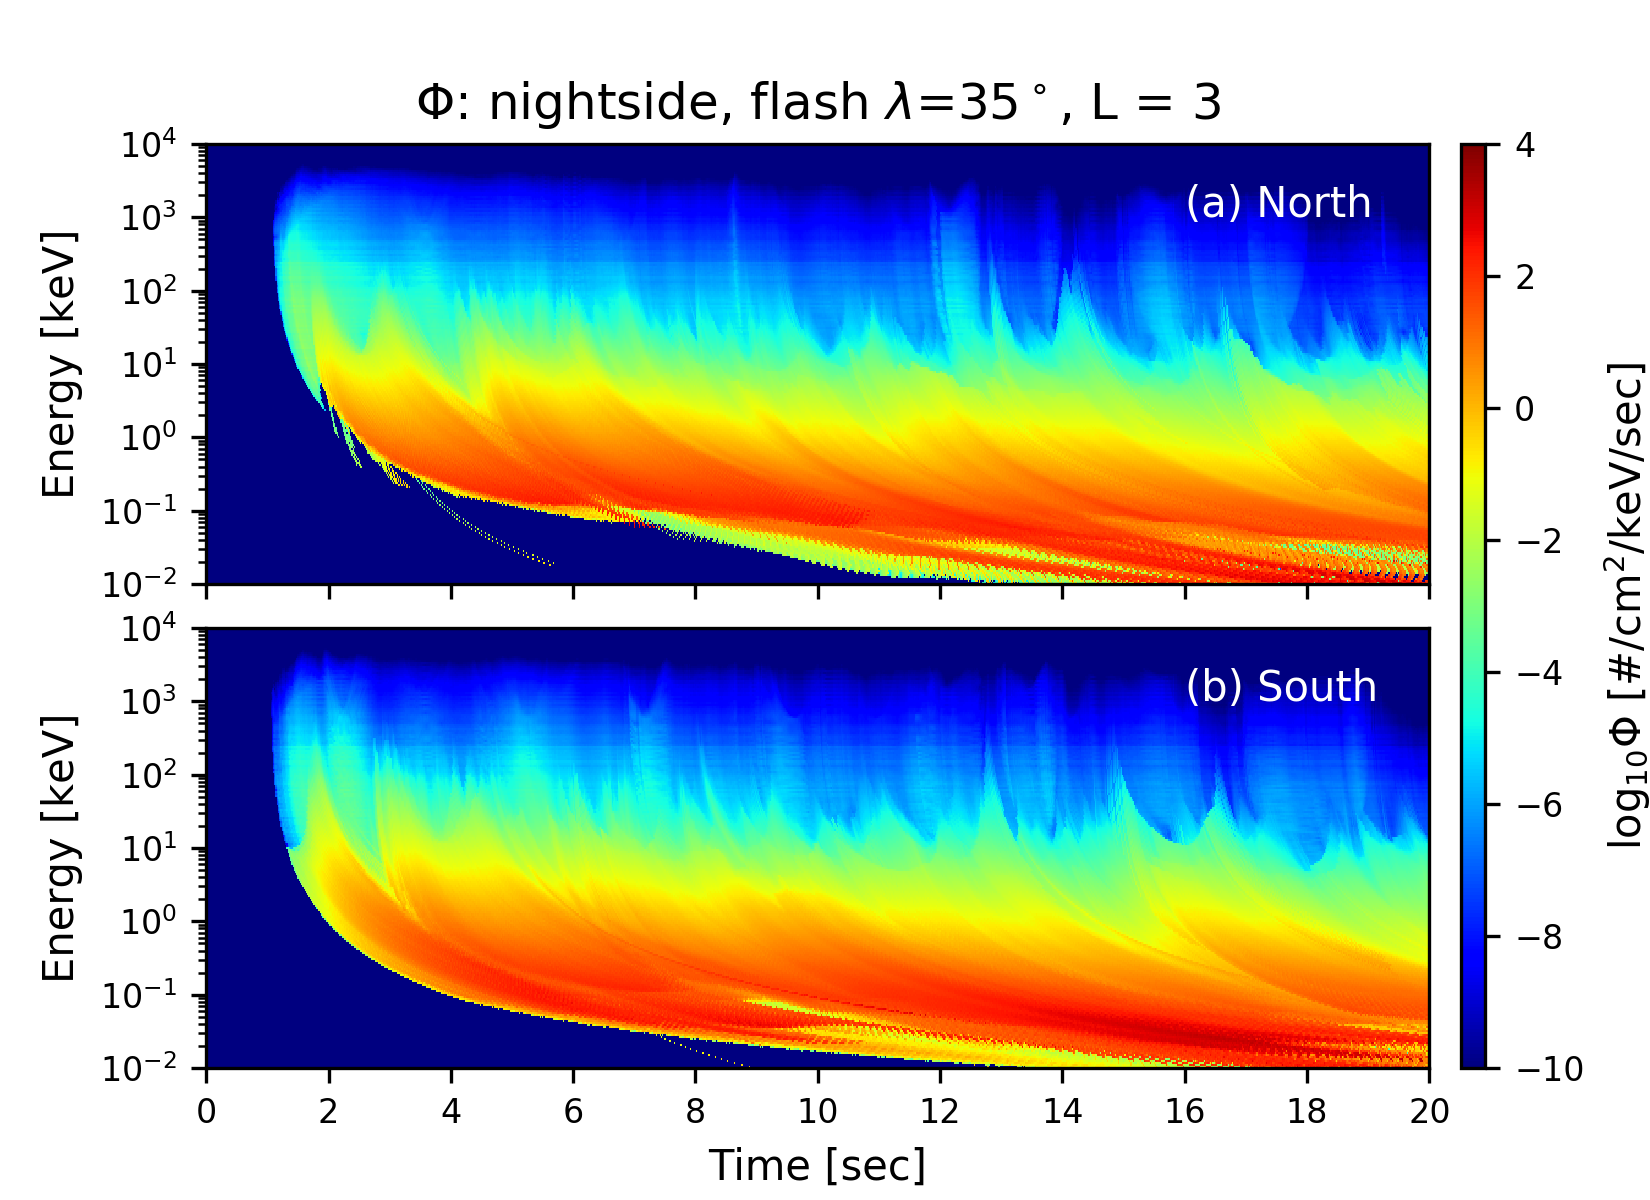
\includegraphics{figures/phi_E-t_spectra.png}
\caption[Precipitating flux density E-t spectra for $\lambda_s=35^\circ$ and L=3]{Precipitating flux density $\Phi(E,t)$ along a fieldine with L=3, for a 10 kA flash at $\lambda_s=35^\circ$ latitude, through a nightside ionosphere at \kp{}=0. Scattering is centered directly over the input flash longitude, within a width of $\pm0.25^\circ.$}
\label{fig:phi_E-t_spectra}
\end{center}
\end{figure}

Equation \eqref{eqn:convolution} is evaluated analytically using a linear expansion of $G(E,t,\alpha)$ about $\alpha = \alpha_{lc}$ (\cite{Bortnik2005}, Figure 5.8, section d).

%The resulting convolution gives a perturbed distribution of pitch angles for each energy band $f_\mathrm{p}(E,t,\alpha)$, a portion of which is within the loss cone. To convert the loss-cone pitch angle distribution to a number (or energy) electron flux density $\Phi_\mathrm{p}(E,t,\alpha)$, we apply the formula from \cite{Chang1983}:
%
%\begin{equation}
%\Phi_\mathrm{p}(E,t,\alpha) = \frac{f_\mathrm{p}(E,t,\alpha)v^2}{m \gamma^3}
%\end{equation} 
%
%where $v$, $\gamma$, and $m$ are the velocity, Lorentz correction factor, and mass of a particle. 
Total fluxes are derived by integrating over the loss cone solid angle, again following \cite{Bortnik2005}, including a $\sin^{-2}\alpha_{lc}$ term to account for fieldline focusing, and $\cos\alpha$ to select the plane perpendicular to $B_0$:

\begin{eqnarray}
\Phi(E,t)& = &\frac{1}{\sin^2\alpha_{lc}}\int_0^{2\pi}\int_0^{\alpha_{lc}}\Phi_\mathrm{p}(E,t,\alpha) \cos\alpha \sin\alpha\,d\alpha\,d\phi \\
&=& \frac{1}{\sin^2\alpha_{lc}} \int_0^{\alpha_{lc}}\Phi_\mathrm{p}(E,t,\alpha) \sin 2\alpha\,d\alpha
\label{eqn:phi}
\end{eqnarray}

Figure \ref{fig:phi_E-t_spectra} shows an example $\Phi(E,t)$ matrix, as calculated with a 10-kA flash at $\lambda_s=35^\circ$, for L=3.


Finally, number flux N and energy flux Q can be calculated by integrating over a desired energy band of interest ($E_1, E_2$):

\begin{eqnarray}
N(t) &=& \int_{E_1}^{E_2} \Phi(E,t)\,dE \\
Q(t) &=& \int_{E_1}^{E_2} E \Phi(E,t)\,dE
\end{eqnarray}



\section{LEP stencils and the behavior of a single flash}
\label{section:lep_stencils}
Having developed a method of computing the precipitating electron energy-time spectrum along a single fieldline, we can compute the global precipitation flux due to terrestrial lightning, using a similar ``stencil'' structure as in Chapter \ref{chapter:power}. We then sum over the time axis to compute the electron flux density in equation \eqref{eqn:phi} for each flash, repeating the calculation for a grid of output L-shells and longitudes, for an array of input latitudes, MLT, and \kp{}.

Table \ref{tab:stencil_params} lists the various parameters used in the stencil simulation. The collection of guide rays are the same as those in chapter \ref{chapter:power}.


\begin{table}[t]
\caption{Stencil Simulation Parameters}
\begin{center}

\begin{tabular}{c|c}
Grid and Interpolation Parameters: \\
\hline \hline
Fine-scale Frequencies & 50 \\
Output L-shell range & 1.2 - 8 \\
Output L-shell spacing & 0.2 \\
Output longitude offsets & \{0, 0.5, 1, 1.5, 2, 5, 10, 20\} \\
Threshold distance from flash & 1000 km \\
 & \\
Resonant Interaction Parameters: \\
\hline \hline
Fieldline latitude spacing & 1$^\circ$ \\
Resonant modes & \{ -5 .. 5 \} \\
Energy bands & 256, log-spaced between 10 eV and 10 Mev\end{tabular}
\end{center}
\label{tab:stencil_params}
\end{table}%

After integrating over the time axis, the resulting stencils each have dimensions (lat $\times$ lon $\times$ energy), for both the northern and southern hemispheres. Figure \ref{fig:precip_stencils} shows a set of energy-integrated number flux stencils for a variety of input latitudes and \kp{} for a 10kA, nightside flash. Figure \ref{fig:precip_stencils_day} shows the corresponding stencils for the dayside.

\begin{figure}[]
\begin{center}
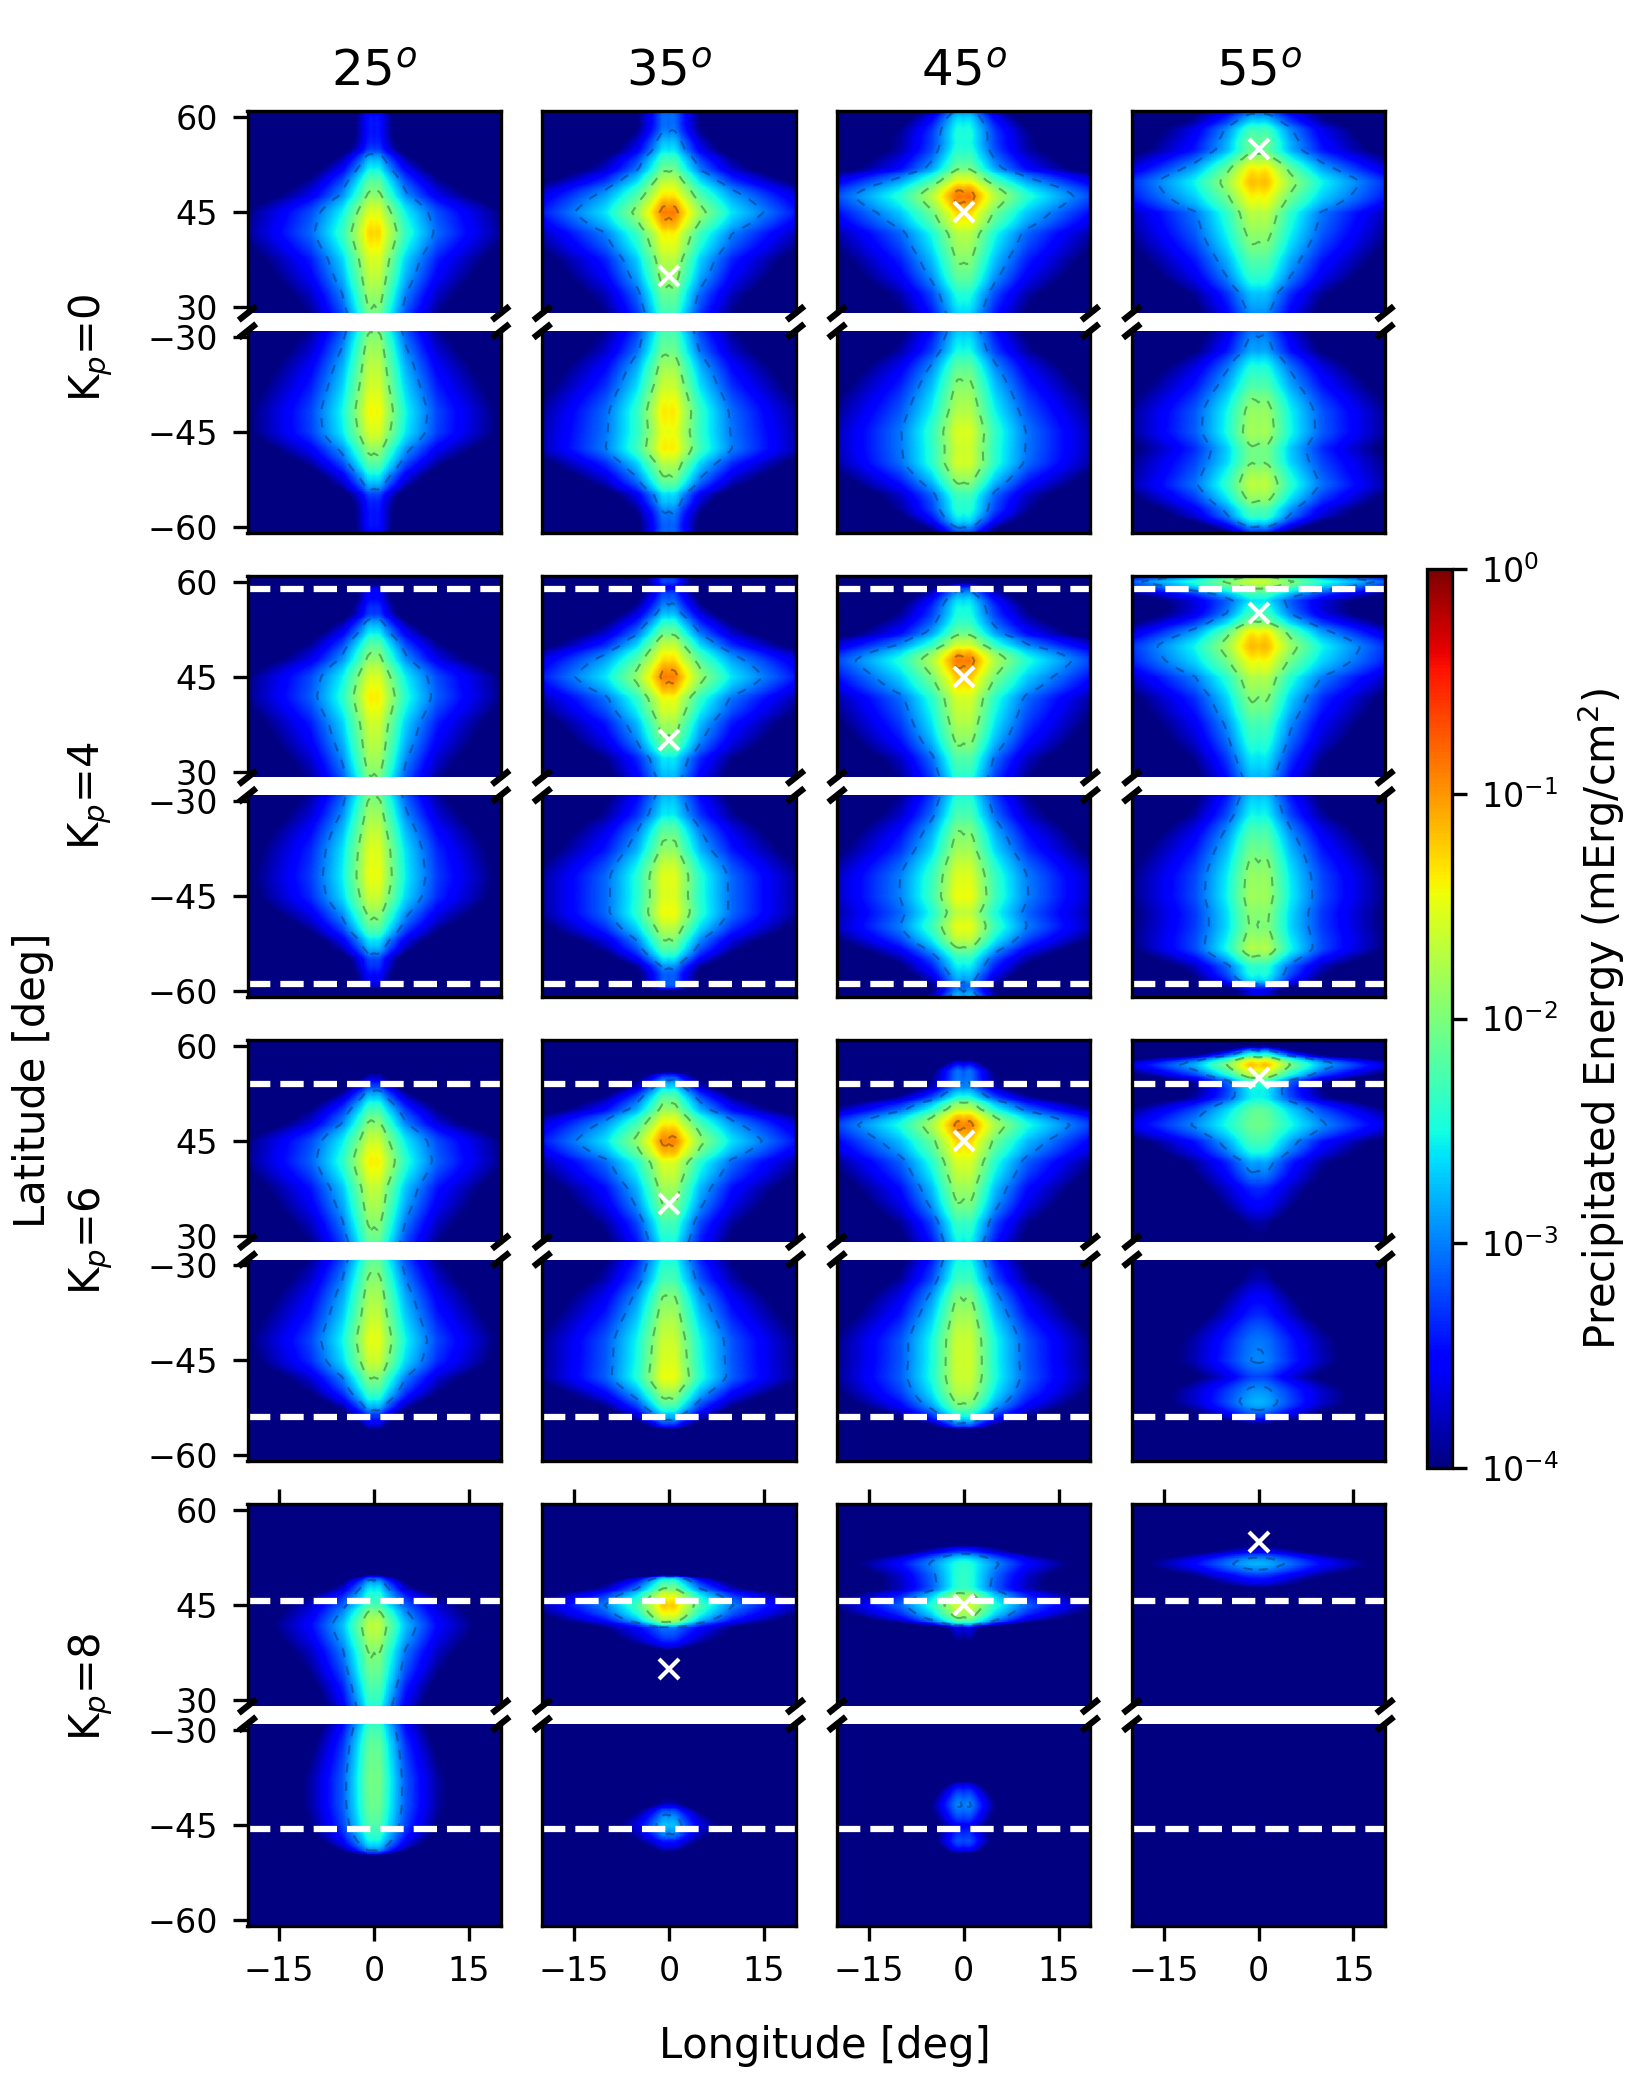
\includegraphics{figures/energy_stencils_nightside_v2.png}
\caption[Precipitating flux density stencils for a range of input latitudes and magnetospheric conditions (nightside)]{Precipitating energy density stencils from a maximally-populated radiation belt model, for a range of flash latitudes and magnetospheric conditions, for a 10 kA nightside flash. The location of the plasmapause is marked with a dashed white line, along the northern and southern hemispheres. The flash location is marked with a white X.}
\label{fig:precip_stencils}
\end{center}
\end{figure}

\begin{figure}[]
\begin{center}
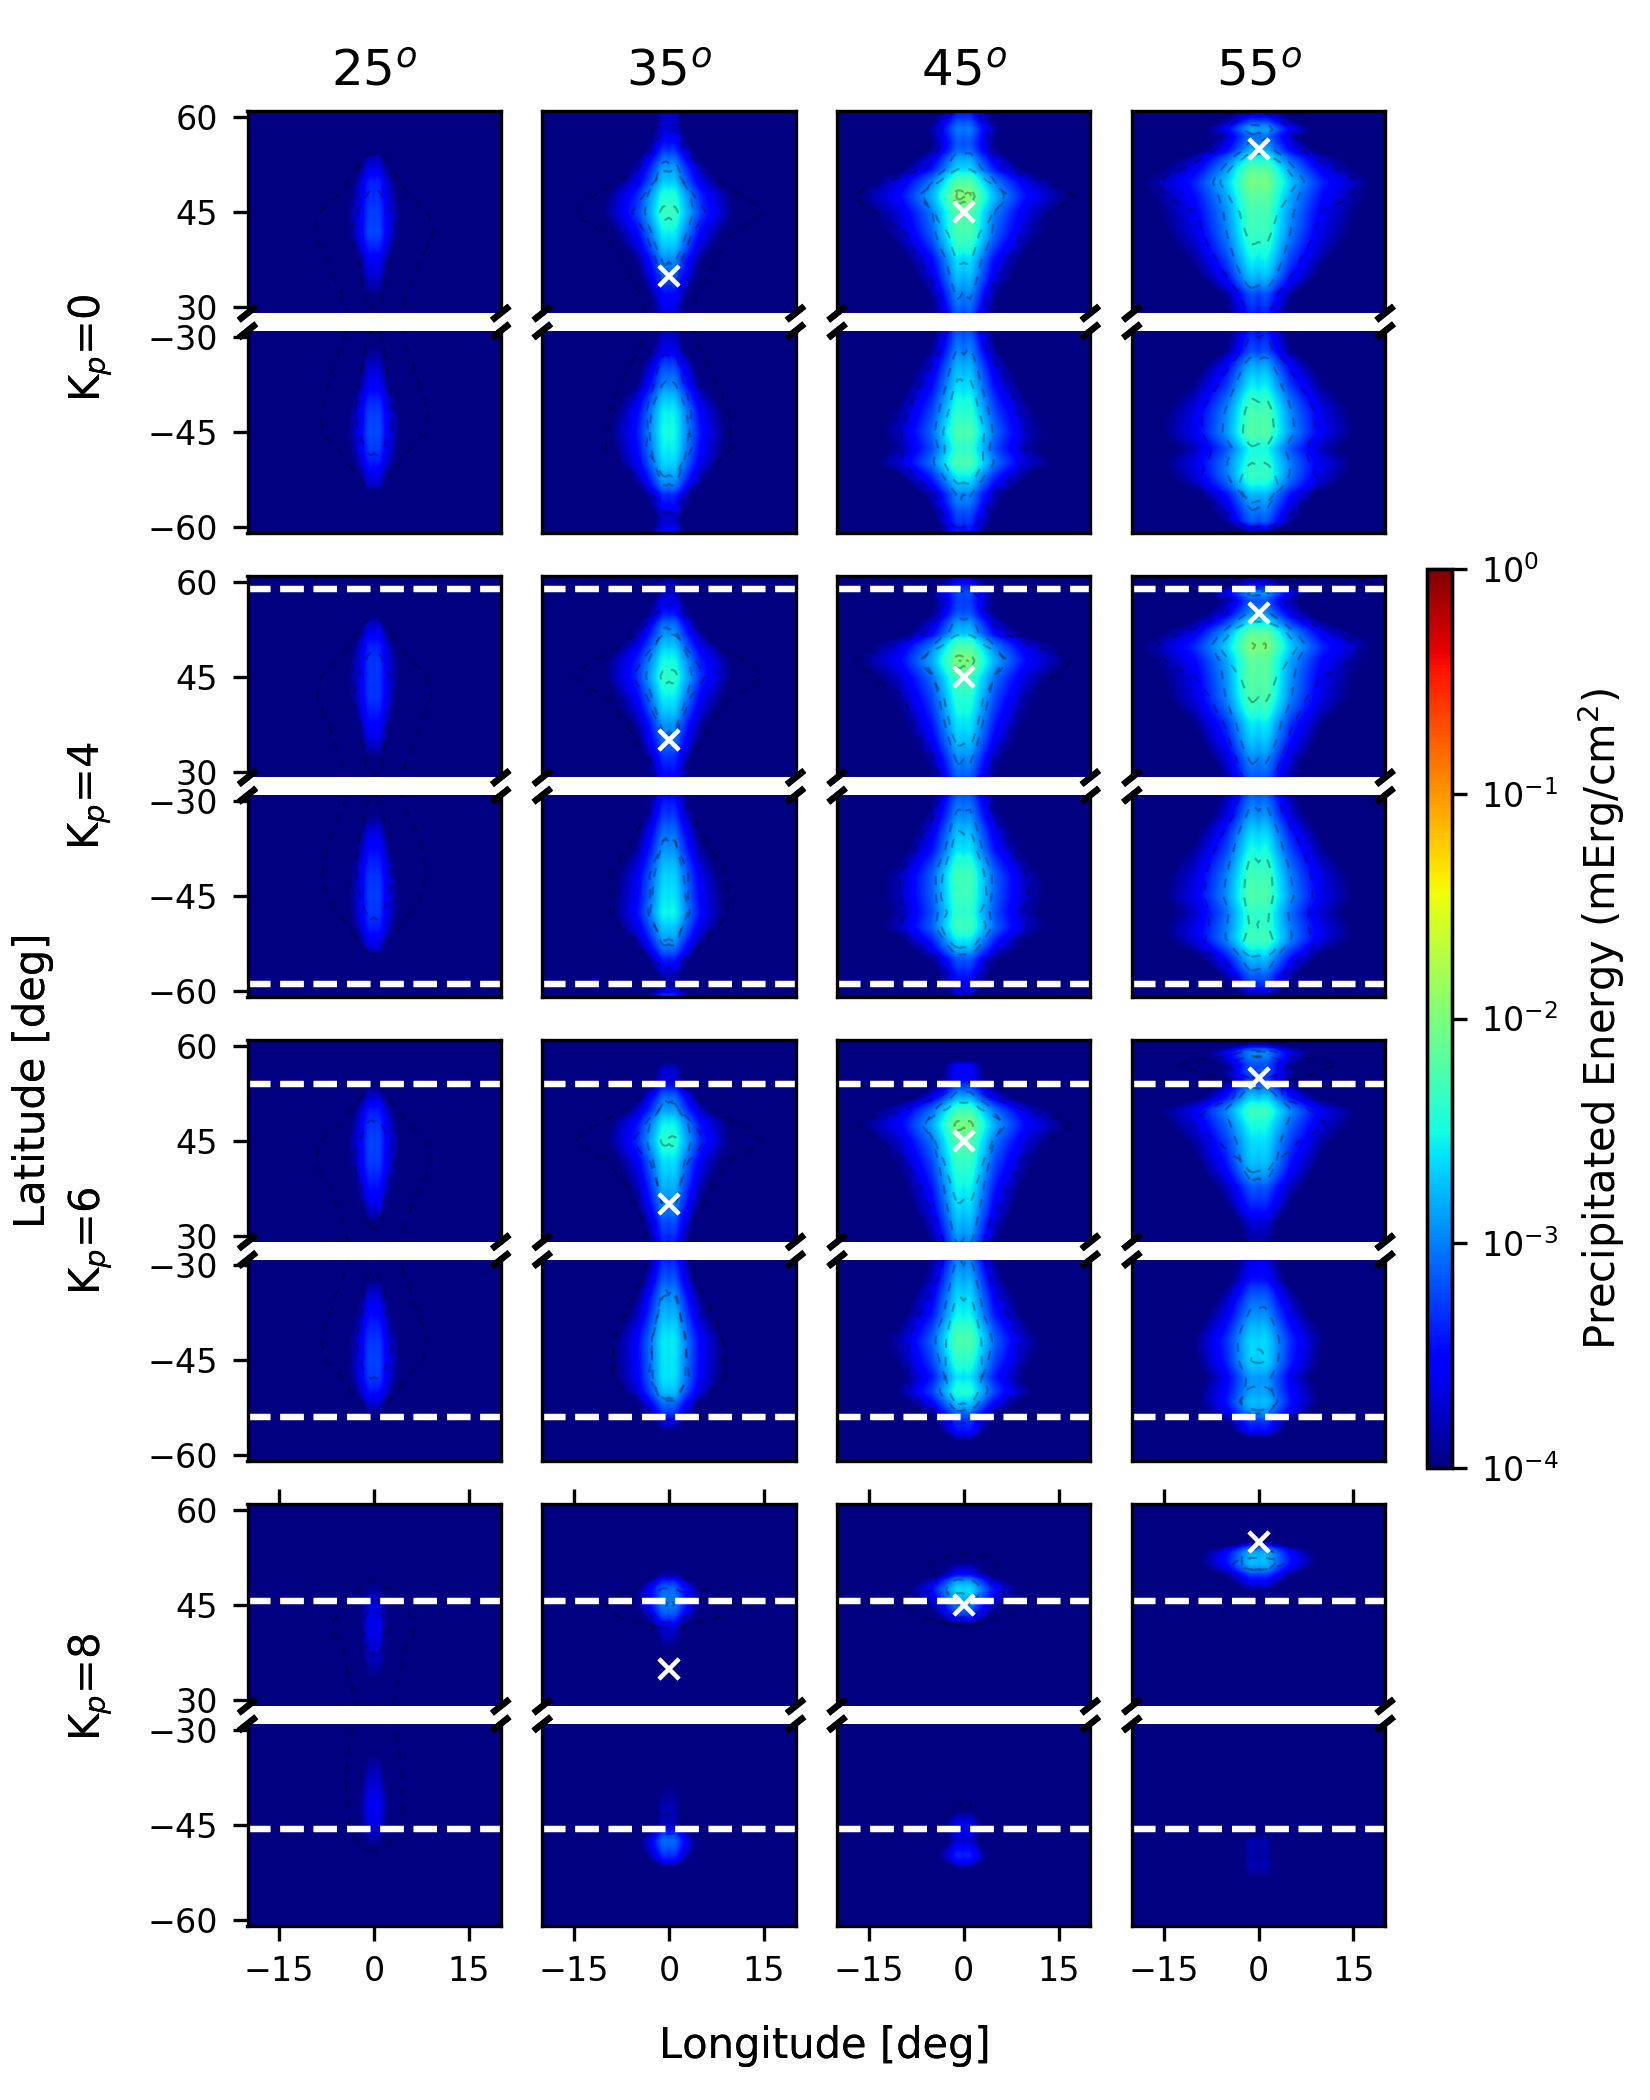
\includegraphics{figures/energy_stencils_dayside_v2.png}
\caption[Precipitating flux density stencils for a range of input latitudes and magnetospheric conditions (dayside)]{Precipitating energy density stencils from a maximally-populated radiation belt model, for a range of flash latitudes and magnetospheric conditions, for a 10 kA dayside flash. The location of the plasmapause is marked with a dashed white line, along the northern and southern hemispheres. The flash location is marked with a white X.}
\label{fig:precip_stencils_day}
\end{center}
\end{figure}

By integrating over latitude and longitude, we can compute the total energy precipitated from a single flash, as shown in Figure \ref{fig:total_energy_per_stencil}. A 10-kA flash precipitates on the order of 1 to 10 kJ on the nightside, and 1 to 1000 J on the dayside.

\begin{figure}[]
\begin{center}
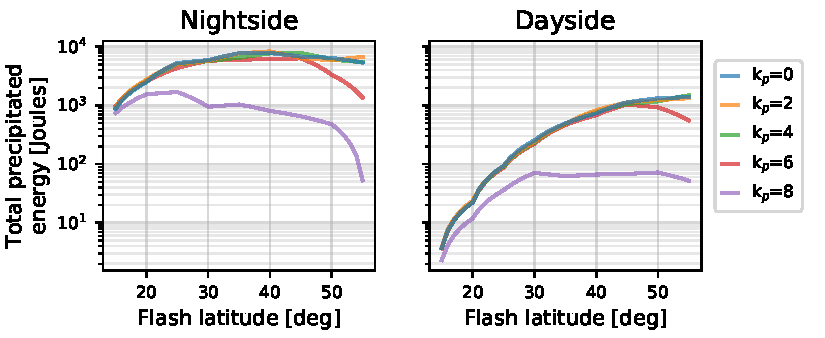
\includegraphics{figures/total_energy_vs_latitude.pdf}
\caption[Total precipitated energy for a single flash]{Area-integrated precipitation for a single 10 kA flash vs flash latitude, for a variety of magnetospheric conditions. Totals include precipitation in both hemispheres.}
\label{fig:total_energy_per_stencil}
\end{center}
\end{figure}

Several trends are apparent in figures \ref{fig:precip_stencils} and \ref{fig:precip_stencils_day}: First, it is apparent that increased \kp{} has little impact on precipitation, up until high activity (\kp{}$ > \sim 6$). We can attribute this to our plasmasphere density model, which is consistent across \kp{} values within the plasmapause. Generally, if a flash is launched within the plasmapause (at a latitude lower than that of the plasmapause), then the rays experience relatively little attenuation due to Landau damping in the cold medium, and reflect back and forth several times. Rays launched outside the plasmapause are attenuated much more quickly. The sharp gradient of the plasmapause constrains energy within the plasmasphere, as indicated by the sharp dropoff of precipitation around the plasmasphere latitude. At the highest values of \kp{}, the plasmapause is brought in to L $\sim$, about 45$^\circ$, at which point substantial energy is launched outside the plasmapause (and quickly damped), or is very strongly deflected by the plasmapause gradient. The effect of the plasmapause is consistent in both the nightside and dayside stencils.

Examining the dayside stencils in Figure \ref{fig:precip_stencils_day}, the increased attenuation of the ionosphere becomes apparent, notably at lower-latitude flashes. The effect of both ionosphere attenuation and of the lower-latitude plasmapause is apparent when looking at the integrated totals in Figure \ref{fig:total_energy_per_stencil}.

Precipitation is not always symmetric between the northern and southern hemispheres. We can attribute any asymmetry in total flux to the relative efficiency of each resonant mode. Higher-order modes (m = $\pm 1$, $\pm 2$...) are symmetric, with the positive calculation resonating with particles moving in one direction, and the negative with particles moving in the opposite. However, the lowest resonant mode (m = 0) interacts only with counterstreaming particles. Accordingly, precipitation is strongest at the same hemisphere as the incident flash.

In both figures \ref{fig:precip_stencils} and \ref{fig:precip_stencils_day}, precipitation is strongest along a $\sim 0.8^\circ$ offset in longitude, which results from the $\sin^2\theta$ term in equation \eqref{eqn:farfield_power_fd}. In this case, $\theta$ represents the elevation angle from the flash to the lower ionosphere (taken to be 100 km), which is maximized at $\theta = 45^\circ$. The result is a central null in radiated energy directly above the flash, and maximal radiated energy offset by 100 km in the longitudinal direction.

An additional point of interest is the ratio of precipitated energy in Figure \ref{fig:total_energy_per_stencil} vs the radiated energy above the ionosphere in Figure \ref{fig:illumination_totals}. Radiation on the order of megajoules will induce precipitation several orders of magnitude lower in energy. 

Finally we can examine the energy spectrum of precipitating electrons, as shown in Figure \ref{fig:stencil_energy_spectrum}. As in the precipitation stencil maps, increasing \kp{} has little effect until very active conditions. The flux is dominated by lower-energy electrons, owing to the stronger scattering of the lowest resonant mode (also visible in Figure \ref{fig:phi_E-t_spectra}).

\begin{figure}[t]
\begin{center}
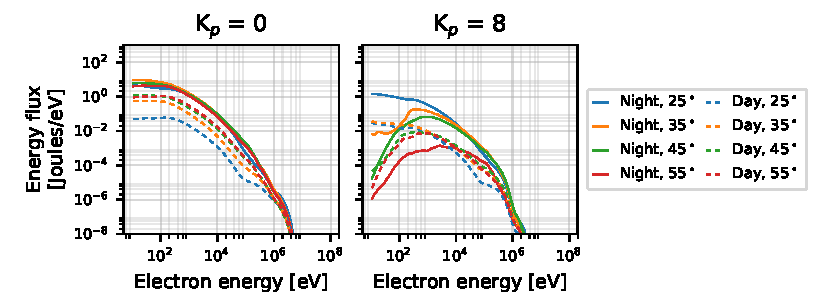
\includegraphics[clip]{figures/stencil_energy_spectrum.pdf}
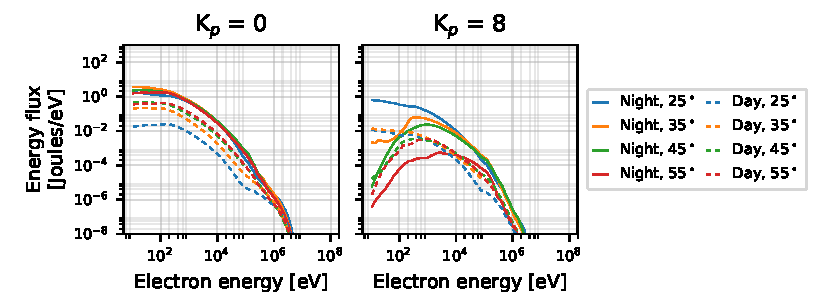
\includegraphics[clip]{figures/stencil_energy_spectrum_AE8MIN_flux_0.pdf}
\caption[Energy spectrum of LEP stencils]{Energy spectrum of precipitating electrons, for \kp{}= 0 and 8, for a range of input latitudes, for day and night. Fluxes are drawn from the AE8MAX population model in the top row, and from the AE8MIN population model in the bottom row.}
\label{fig:stencil_energy_spectrum}
\end{center}
\end{figure}


\section{Coordinate deformation}
The stencils in section \ref{section:lep_stencils} are computed using a dipole magnetic field, and the simplified GCPM model, both to reduce computational complexity and to better generalize to multiple longitudes. However, we can approximate the effect of a more-complex magnetic field model via a coordinate transformation, in which we rotate input coordinates to an equivalent dipole-model coordinate, and perform an inverse operation on the stencil output. On the stencil output, this approximation is justified by noting that trapped electrons are bound to their respective field lines, regardless of model used. Justification on the input side (deforming the input coordinates of a lightning flash) is less-concrete, but still a reasonable assumption. First, experimentation with the raytracer reveals that, given a longitudinally-symmetric plasma density model, rays generally follow the longitude deviation of the magnetic field model. Second, while the IGRF and Dipole models differ greatly in its footprint on the ground (as in Figure \ref{fig:Lshell_example}), within the plasmasphere the two models have reasonable agreement (as in Figure \ref{fig:fieldline_example}).

The \emph{Corrected Geomagnetic Coordinate} (CGM) \citep{Hakura1965} system is especially well-suited for this task. CGM coordinates are defined by fieldline tracing between the IGRF and Dipole models. To transform from geographic to CGM coordinates, we first trace a fieldline using IGRF from the surface, up to its intersection with the geomagnetic equatorial plane. We then follow the dipole model back down to the surface, to get an equivalent dipole-model coordinate. The inverse transformation is accomplished by following the dipole field line back up to the equator, and the IGRF model down to its footprint \citep{Laundal2016}.

Field line tracing is a computationally-intensive task for a coordinate transformation tool. Historically, researchers relied on precomputed lookup tables and interpolation. The Altitude-Adjusted CGM (AACGM) model \citep{Baker1989, Shepherd2014} uses a spherical-harmonic fit to rapidly transform between CGM and MAG coordinates.

\begin{figure}[t]
\begin{center}
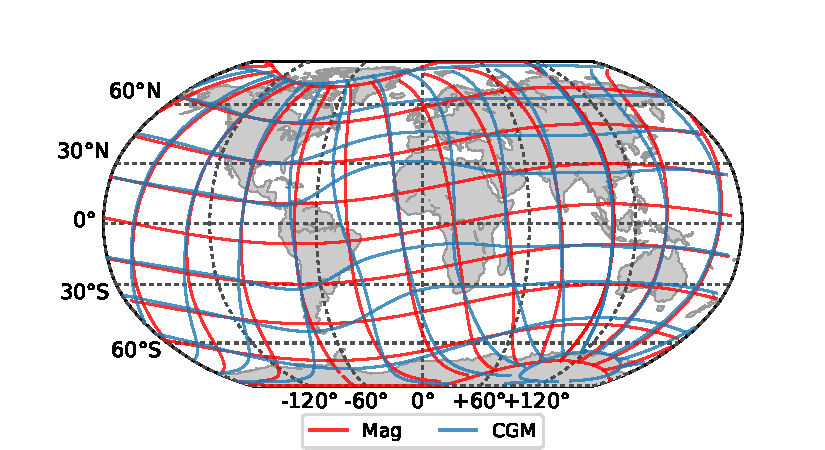
\includegraphics{figures/CGM_globe_comparison.pdf}
\caption[Comparison of Magnetic Dipole (MAG) and Corrected Geomagnetic (CGM) coordinates]{A comparison between Magnetic Dipole (MAG) and Corrected Geomagnetic (CGM) coordinates. Corrected Geomagnetic coordinates are obtained by following a magnetic field line, as defined by IGRF, from an input point to its intersection with the magnetic dipole equator. The CGM latitude and longitude are then obtained by following the dipole field line to its footprint on the Earth's surface. Contours are spaced every $20^\circ$ in geomagnetic latitude, and $30^\circ$ in geomagnetic longitude.}
\label{fig:CGM_globe_comparison}
\end{center}
\end{figure}    

CGM coordinate systems are undefined at some regions near the geomagnetic equator, due to the fact that some IGRF fieldlines may never intersect with it. In these cases, approximate models are often used. \cite{Baker1989} simply omitted geomagnetic latitudes within $\sim 24^\circ$ of the equator from their study; subsequent researchers have performed spline fits and interpolation to further reduce the undefined region.

We use the AACGMv2 algorithm and implementation from \cite{Shepherd2014}, available at \emph{http://superdarn.thayer.dartmouth.edu/aacgm.html}. Figure \ref{fig:CGM_globe_comparison} compares MAG and AACGM contours on a geographic map.

Figure \ref{fig:CGM_vs_MAG_GLD} shows the relative difference between GLD average current density using MAG coordinates only, vs using the AACGM coordinate transform.



\begin{figure}[]
\begin{center}
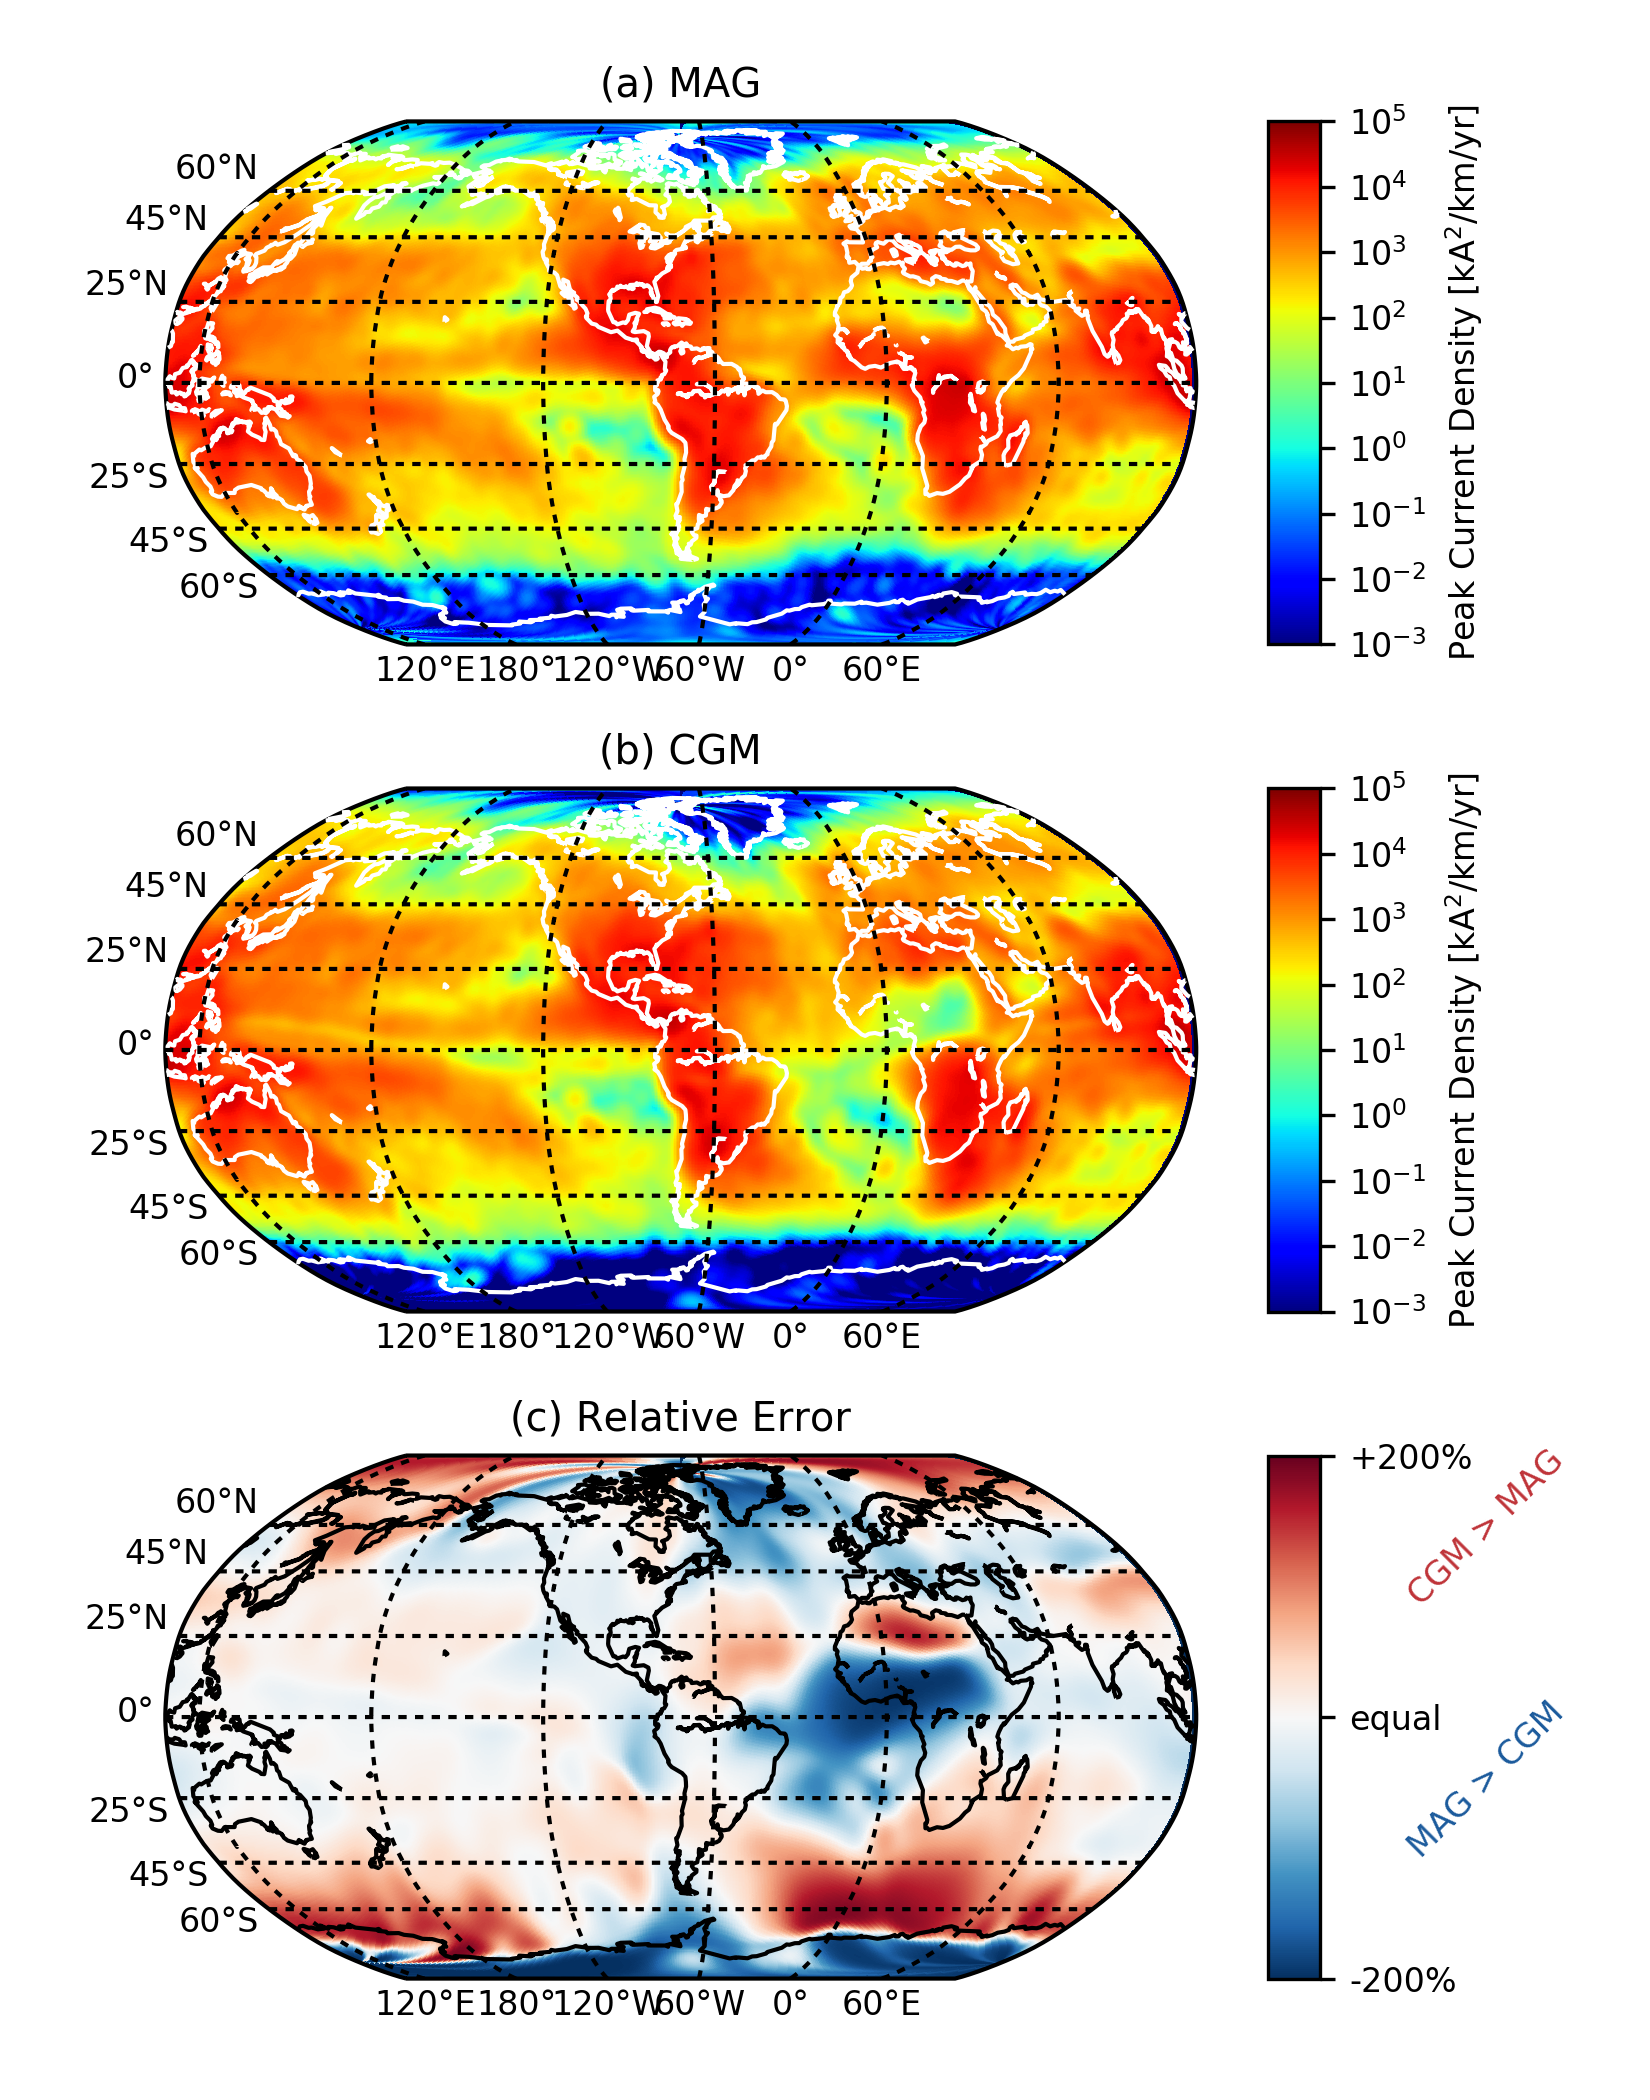
\includegraphics{figures/GLD_CGM_vs_MAG_comparison.png}
\caption[GLD average peak current density, adjusted using AACGM coordinates]{Average lightning activity, weighted by peak current intensity, as measured by the GLD360 dataset. Data is averaged from August 2014 through July 2017. (a) the GLD360 data, in geographic coordinates. (b) the GLD360 data, shifted to its equivalent coordinates using the AACGM coordinate transform. (c) the relative error between the two coordinate frames.}
\label{fig:CGM_vs_MAG_GLD}
\end{center}
\end{figure}


% Our study already excludes these latitudes on the basis that below $\sim 20^\circ$ geomagnetic latitude, field lines do not exit the ionosphere at their apex.


\section{Global and Seasonal Energy Fluxes}

Having computed the precipitation for a single flash across a variety of input parameters, we can examine global energy deposition by shifting, scaling, and summing the LEP stenciles according to the GLD360 lightning dataset. The resulting electron precipitation is heavily dependent on the population of radiation belt electrons; rather than leverage historical data, we provide two estimates, using the AE8 model for maximal and minimal filling, in effort to determine the upper and lower bounds on precipitation. 

LEP stencils are computed using the parameters in table \ref{tab:stencil_params}. Stencils are computed for canonical 10 kA flashes, in 5$^\circ$ steps in latitude, between 15$^\circ$ and 55$^\circ$, for dayside and nightside (MLT = 12 and 0 respectively), for an array of \kp{} = \{0, 2, 4, 6, 8\}. The resulting stencils are then interpolated onto a fixed 0.5$^\circ$x0.5$^\circ$ grid in geomagnetic latitude and longitude, and for all valid values of \kp{} (0 - 9 in $\sim$ 0.3 steps). Noting the relatively quick transition at the day/night terminator, we bin each flash in the GLD360 dataset into dayside or nightside. The 256 energy bands are summed into 64 sub-bands to reduce memory requirements. 

Figure \ref{fig:global_precip_map_max_min} shows the global average energy precipitation resulting from LEP, for maximum and minimum conditions. Precipitation is integrated over the energy band of interest (10 eV - 10 MeV), and averaged over a three year period between August 2014 and July 2017. We use historical data for \kp{}, which is reported in three-hour segments.

The pitch-angle scattering model scales linearly with respect to wave amplitude, and therefore scales quadratically with respect to flash peak current. To account for arbitrary peak current values, we scale the resulting precipitation stencils accordingly:

\begin{equation}
\phi(I) = \phi(I_{ref})\frac{I^2}{I_{ref}^2} 
\end{equation}

The two sources of stochasticity in our model are 1) the location and intensity of lightning, and 2) the value of \kp{}. Lightning activity and \kp{} are generally uncorrelated, as \kp{} is driven by activity within the magnetosphere, and lightning activity by terrestrial weather patterns. As shown in figures \ref{fig:precip_stencils} and \ref{fig:precip_stencils_day}, fluctuations in \kp{} have little effect on our precipitation model in most situations (\kp{}$ < 6$). Unexplored in this work, however, is the correlation between radiation belt filling conditions and \kp{}; e.g., radiation belt filling events generally occur alongside geomagnetically-active conditions, in which \kp{} will be high.

\begin{figure}[]
\begin{center}
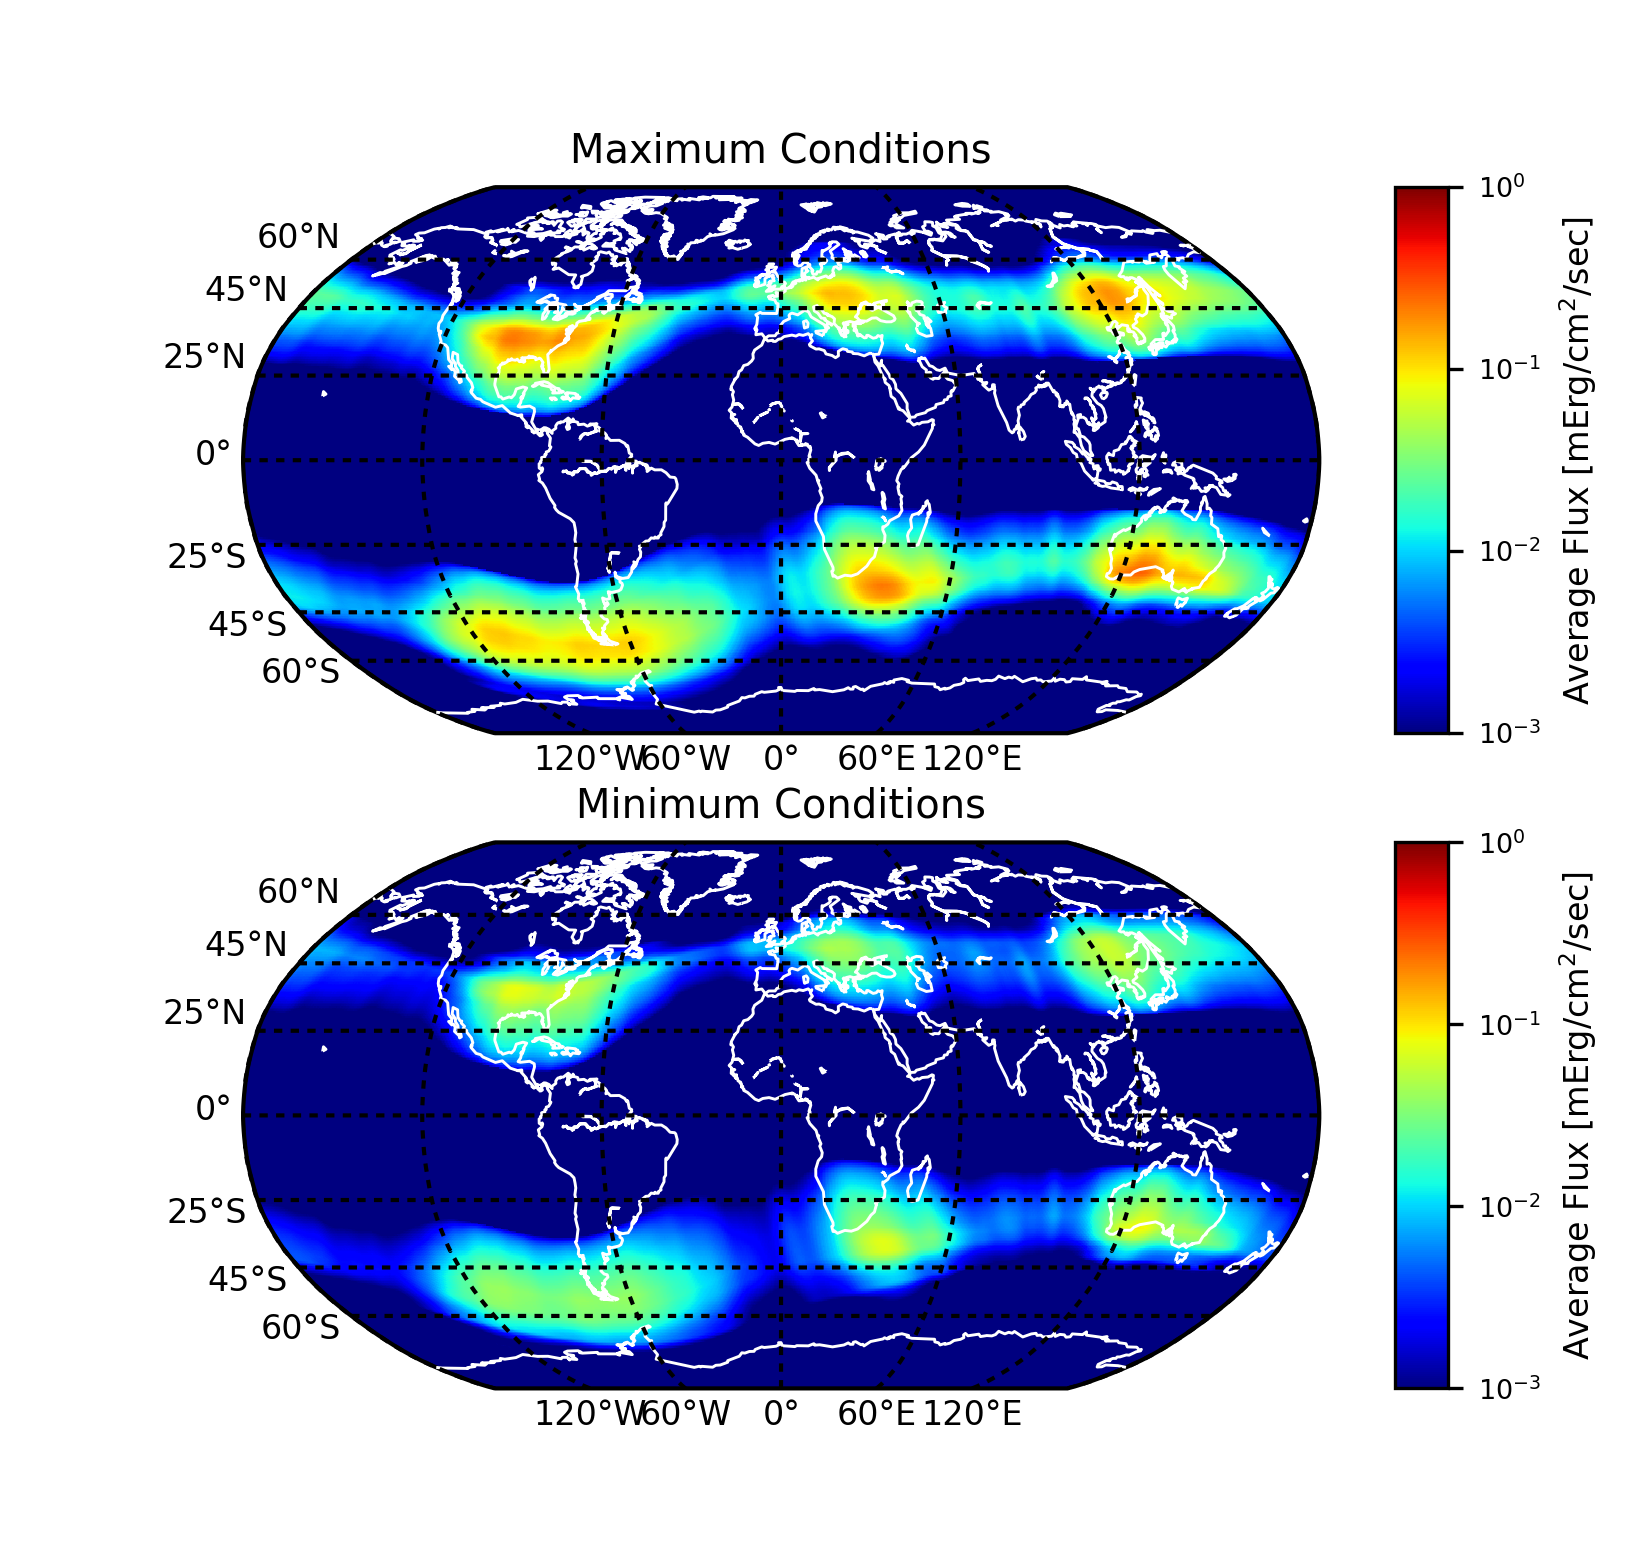
\includegraphics{figures/global_precip_map_max_min.png}
\caption[Global energy deposition ``hot spots'' for maximal and minimal radiation belt populations]{Time-averaged energetic electron precipitation ``hot spots'', for the GLD360 dataset, between August 2014 and July 2017. Total energy is shown, integrated between 10 eV and 10 MeV. }
\label{fig:global_precip_map_max_min}
\end{center}
\end{figure}

By integrating over latitude and longitude, rather than time, we can examine any seasonal trends which may be present. Figure \ref{fig:seasonal_precip_rates_global} shows the global energy flux in kilowatts, across the globe, as a function of time, for maximal and minimal filling conditions. The global energy deposition rate shows very weak seasonal dependence, and can range from a few kilowatts to several megawatts. The disperse energy deposition rate suggests that LEP is not a prominent driver of energy in the upper atmosphere. However, sporadic energy deposition due to LEP is measurable by sub-ionosphere VLF remote sensing \citep{Inan1990, Johnson1999, Cotts2011}, and may still be capable of inducing turbulence in the upper ionosphere, either by precipitating particles or the interaction of the upgoing whistler wave \citep{Berthelier2008}.

The lack of seasonal dependence, however, suggests that LEP can provide a constant, year-round loss mechanism for radiation belt electrons, especially when considering that radiation belt electrons can drift in longitude around the Earth, on timescales of minutes to days \citep{Walt1994}, and can thereby interact with lightning activity across the globe.

\begin{figure}[ht]
\begin{center}
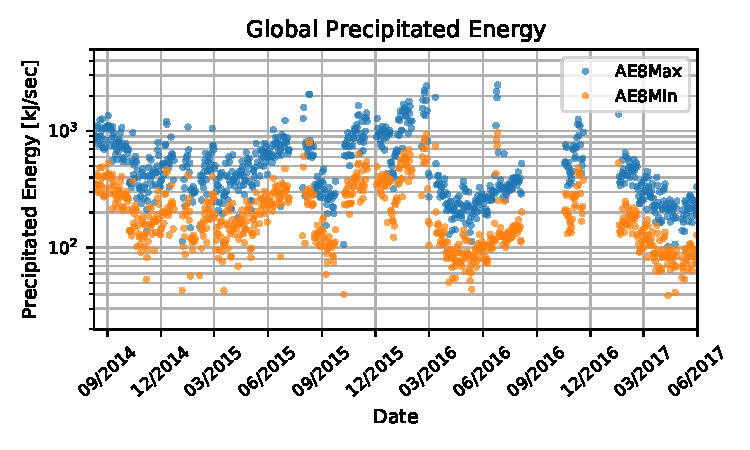
\includegraphics{figures/seasonal_precip_rates_global.pdf}
\caption[Global energy deposition due to LEP]{Global average energy deposition due to LEP. Precipitation is integrated across the globe, for energetic electrons between 10 eV and 10 MeV.}
\label{fig:seasonal_precip_rates_global}
\end{center}
\end{figure}
\begin{figure}[h]
\begin{center}
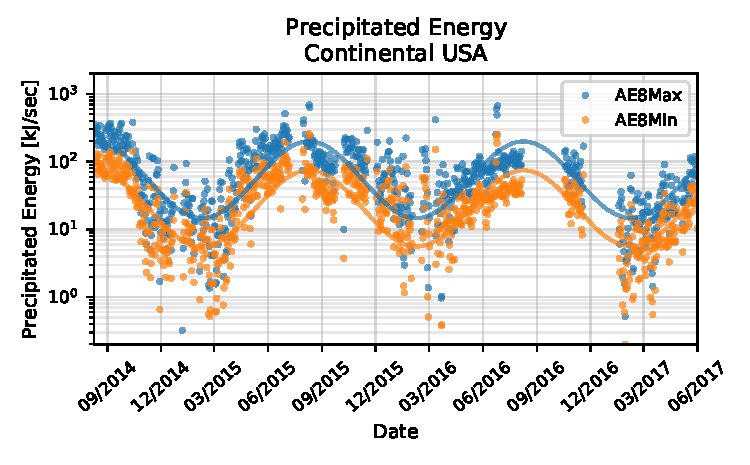
\includegraphics{figures/seasonal_precip_rates_US_only.pdf}
\caption[Global energy deposition due to LEP over the continental United States]{Average energy deposition due to LEP over the continental United States (20$^\circ$ to 50$^\circ$ geomagnetic latitude, -50$^\circ$ to +10$^\circ$ geomagnetic longitude). Seasonal variation is much more apparent than in the global integration (Figure \ref{fig:seasonal_precip_rates_global}).}
\label{fig:seasonal_precip_rates_US_only}
\end{center}
\end{figure}

While total global lightning activity is relatively constant, regional lightning is a highly seasonal phenomenon. We can integrate the energetic electron precipitation over the continental United States, to explore seasonal dependence on a finer scale, such as in \cite{Gemelos2009}. Figure \ref{fig:seasonal_precip_rates_US_only} shows the total energy precipitation between 20$^\circ$ - 50$^\circ$ in geomagnetic latitude, and -50$^\circ$ to +10$^\circ$ in geomagnetic longitude (approximately over the continental United States). Narrowing our observation window reveals a much greater seasonal variation, peaking in the summer months, and reaching a minimum in December and January.



\section{Lifetime Estimates}
The previous section examined the energy deposition into the ionosphere due to LEP. Next, we consider the relative effect of LEP as a loss mechanism from the populated radiation belts.

Our precipitation model is linearly proportional to the current population of electrons along a given magnetic fieldline, which results in an exponential loss function, parameterized by a time constant $\tau$:

\begin{eqnarray}
\frac{dN}{dt} & \propto & N \\
\therefore N(t) & = & N_0 \exp{-t/\tau} \\
\frac{dN}{dt} & = & -\frac{N_0}{\tau}\exp{-t/\tau} \\
& = & -\frac{N(t)}{\tau} \\
\tau & = & \frac{N(t=t_0)}{dN/dt\rvert_{t0}}
\label{eqn:tau}
\end{eqnarray}

Once summed over the GLD360 dataset, our model delivers electron losses impinging on a cross-sectional area at 100 km, with units [$\#$/cm$^2$/eV/sec]. To compute the percentage loss, we must determine the number of electrons (per energy) which occupy the fieldline above the same cross-sectional area, resulting in $\tau \sim sec$.

The total electrons along a given fieldline above a cm$^2$ ionosphere patch is computed by integrating the (energy) differential, omnidirectional equatorial flux, such as from the AE8 model. As in the precipitation code, we ascribe a sinusoidal pitch-angle distribution (e.g., Figure \ref{fig:pitchangledistributions}) to the electrons in the omnidirectional flux value. 

The AE8 energy-differential, omnidirectional flux models have units J $\sim$ [$\#$/cm$^2$/sec/ev], which represent the total flux of electrons through a cross-sectional area at the equator, per unit energy. We use a change of variables and integrate over the sinusoidal pitch-angle distribution P(L, $\alpha$), using the relationship in equation \eqref{eqn:bounce_time} to relate an electron's bounce time $\tau_b$ to it's pitch angle $\alpha$ and total kinetic energy $E$.

\begin{equation}
  P(L,\alpha)=\begin{cases}
    \bigfrac{1}{1 - 2\alpha_{lc}/\pi}\sin{\bigfrac{\alpha - \alpha_{lc}}{1 - 2\alpha_{lc}/\pi}}, & \text{$\alpha_{lc} < \alpha < \pi - \alpha_{lc}$}. \unit{rad^{-1}}\\
    0, & \text{otherwise}.
  \end{cases}
\end{equation}


\begin{equation}
 % There's more to this -- I'm not showing the whole integrand after the change of variables and addition of the pitch-angle distribution
N_{0,equator} = \int_0^{\pi/2} J(E)P(L,\alpha) \tau_b(L, \alpha)\,\sin{\alpha}\,\cos{\alpha}\,d\alpha \unit{\#/cm^2/eV}
\end{equation}

We then convert the integrated value $N_0$ from an equatorial cross-sectional area to an equivalent cross-sectional area at the ionosphere, using a ``crunch'' term $C_b$ according to the constricting dipole magnetic field:

\begin{eqnarray}
\epsilon_m &= & \frac{1}{L}(R_E + H_{iono})/R_E \\
C_b & = & \sqrt{1 + 3(1 - \epsilon_m)} / \epsilon_m^3 \\ 
N_{0, iono} &=& C_b\,N_{0, equator} \unit{\#/cm^2/eV}
\label{eqn:fieldline_density}
\end{eqnarray}

In order to examine the effectiveness of LEP across all energies, and avoid numerical issues where the AE8 model values are small, we compute an additional set of stencils, using a uniform radiation belt population, by setting $J(E) = 1$ [1/cm$^2$/sec/ev].  Figure \ref{fig:stencil_energy_spectrum_flat_distribution} shows the precipitated energy distribution from a flat radiation belt population, in the same format as Figure \ref{fig:stencil_energy_spectrum}. The bimodal peaks resulting from the multiple resonant interaction modes are more-readily visible, without the additional loss due to reduced radiation belt populations at higher energies.

\begin{figure}[]
\begin{center}
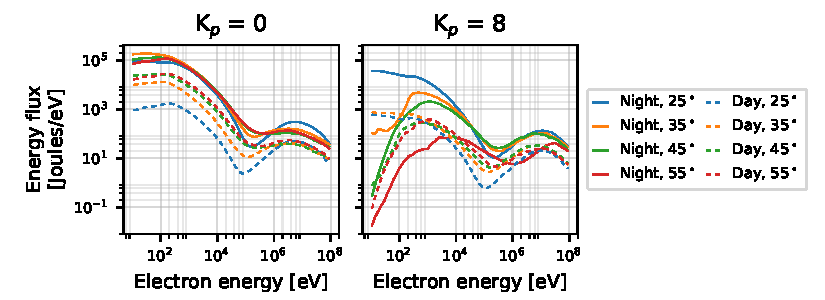
\includegraphics{figures/stencil_energy_spectrum_flat_distribution.pdf}
\caption[Energy spectrum of LEP stencils, drawn from a uniform radiation belt population]{Energy spectrum of precipitating electrons, for \kp{}= 0 and 8, for a range of input latitudes, for day and night, from a uniform (differential flux = 1/cm$^2$/sec/eV) fieldline population.}
\label{fig:stencil_energy_spectrum_flat_distribution}
\end{center}
\end{figure}

We then compute an equivalent precipitation map using the GLD360 dataset, and the flat-distribution stencils. We average the resulting precipitation over all latitudes to obtain a typical flux estimate. The loss timescale, $\tau$, is then obtained using equation \eqref{eqn:tau}, with the fieldline population $N$ computed using equation \eqref{eqn:fieldline_density}, and the loss rate $dN/dt$ given by the global average precipitation estimate, both using the flat distribution for $J$.

Figure \ref{fig:electron_lifetimes} shows the estimated lifetime for radiation belt electrons, subjected solely to LEP-induced losses, versus electron energy and fieldline. Two prominent results are apparent in Figure \ref{fig:electron_lifetimes}: First, we see two enhancement regions, centered at lower energies ($\sim$100 eV), and at higher energies ($\sim$ 10 MeV). We can attribute this bimodal pattern to the preferential energy bands of each resonant mode, as in Figure \ref{fig:stencil_energy_spectrum_flat_distribution}. Interestingly, our model shows a null in precipitation effectiveness in the band between 100 keV and 1 MeV; this band has generally been thought to be the dominant precipitation region (for example, the analysis of a single LEP event in \cite{Voss1998} shows a precipitation spectrum between $\sim$ 100  -- 300 keV. The instrument used, SEEP, measured fluxes binned into 8 energy channels between 2 keV and 10 MeV.) . Second, LEP is only an effective loss mechanism for inner belt and slot-region fieldlines (L $<$ 3), owing to the much much greater volume traversed by higher-L fieldlines.
\begin{figure}[t]
\begin{center}
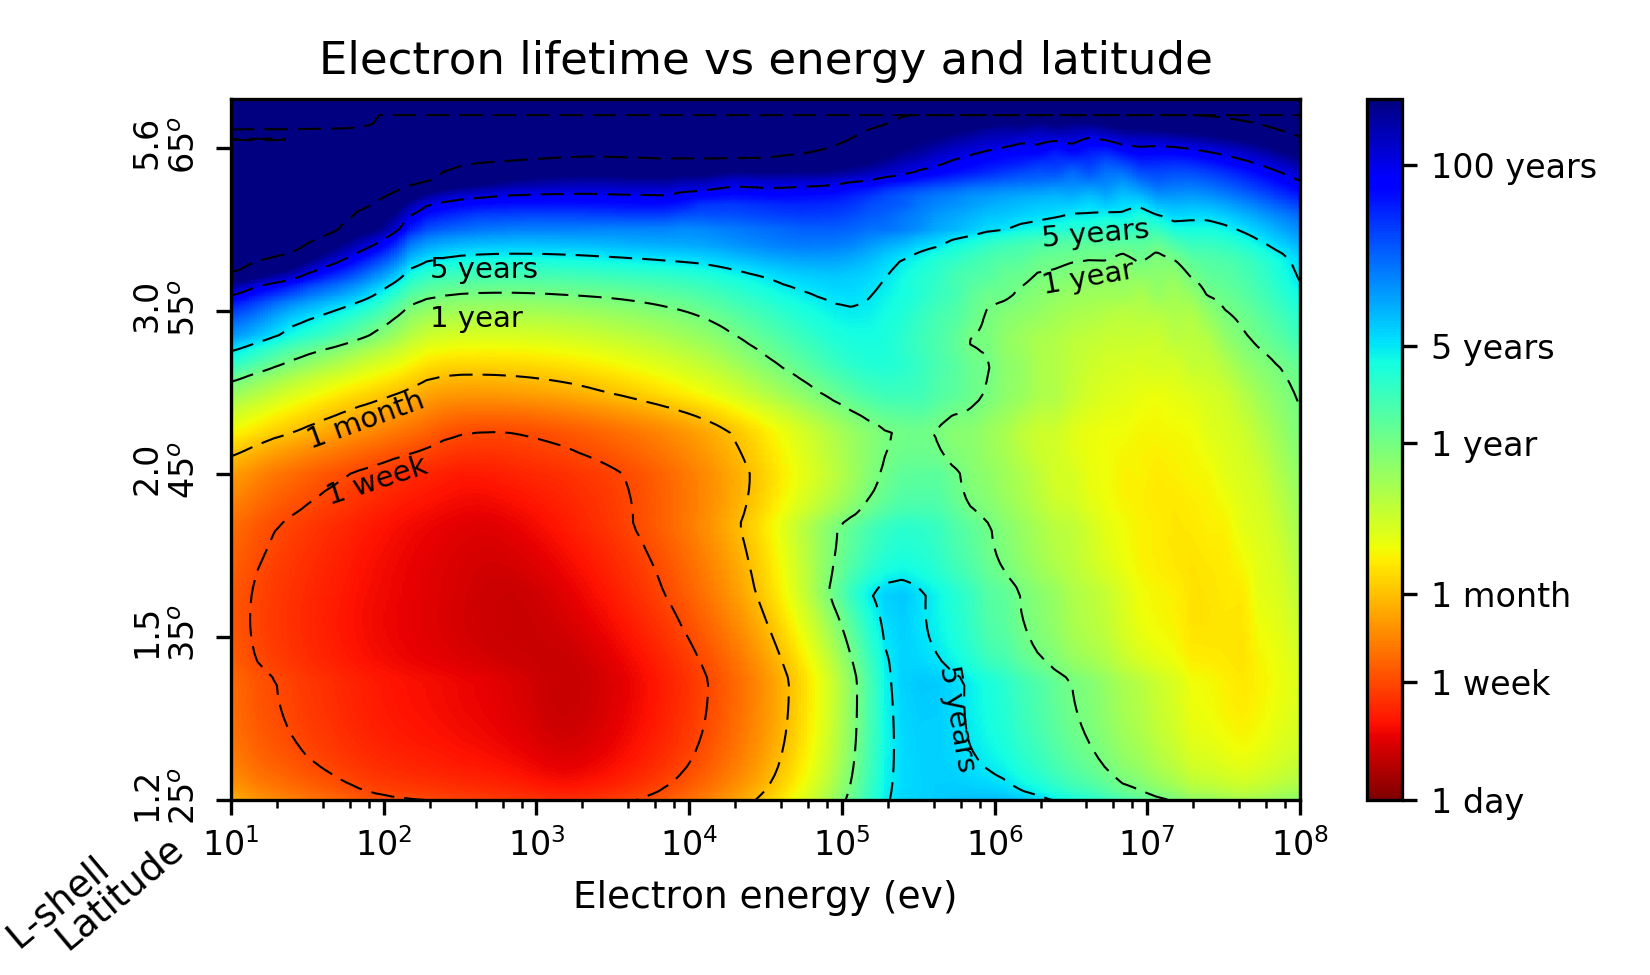
\includegraphics{figures/electron_lifetimes_updated_power_with_labels.png}
\caption[Estimated lifetime of radiation belt electrons subject to LEP losses only]{Estimated lifetimes ($\tau$, the time required for a population to decay by 1/e) for radiation belt electrons subjected solely to LEP-induced losses.}
\label{fig:electron_lifetimes}
\end{center}
\end{figure}


\section{Comparison to other research}
We can compare our resulting precipitation estimates to two related works: \cite{Gemelos2009} used data from the DEMETER spacecraft, along with seasonal lightning fluxes as measured by the NLDN network, to examine seasonal trends in LEP at 126 keV, and \cite{Meredith2007}, which uses \emph{in situ} VLF wave measurements to estimate lifetimes of radiation belt electrons due to various scattering mechanisms (LEP, chorus, hiss), using an incoherent interaction model.

Figure \ref{fig:gemelos_comparison} shows our modeled electron precipitation at 123 keV for August and December, averaged over 2014 - 2017, along with the corresponding northern hemisphere lightning activity as measured by GLD360, to facilitate comparison with \cite{Gemelos2009}, Figure 1. Geographically, our model shows very good agreement with \citeauthor{Gemelos2009}; however our modeled fluxes are several orders of magnitude lower. Possible explanations for the discrepancy in precipitation amplitude are that the DEMETER spacecraft orbited at 710 km altitude, while our fluxes are estimated at 100 km. Additionally, the DEMETER particle detector viewed particles with local pitch angles near $\sim 85^\circ$, and a full-width, half maximum viewing angle of $30^\circ$. Both \citeauthor{Gemelos2009} and \cite{Sauvaud2006} state that at this orientation the detector measures particles within or near the \emph{drift} loss cone, which may be considerably shallower than the bounce loss cone as modeled by our work.

\begin{figure}[]
\begin{center}
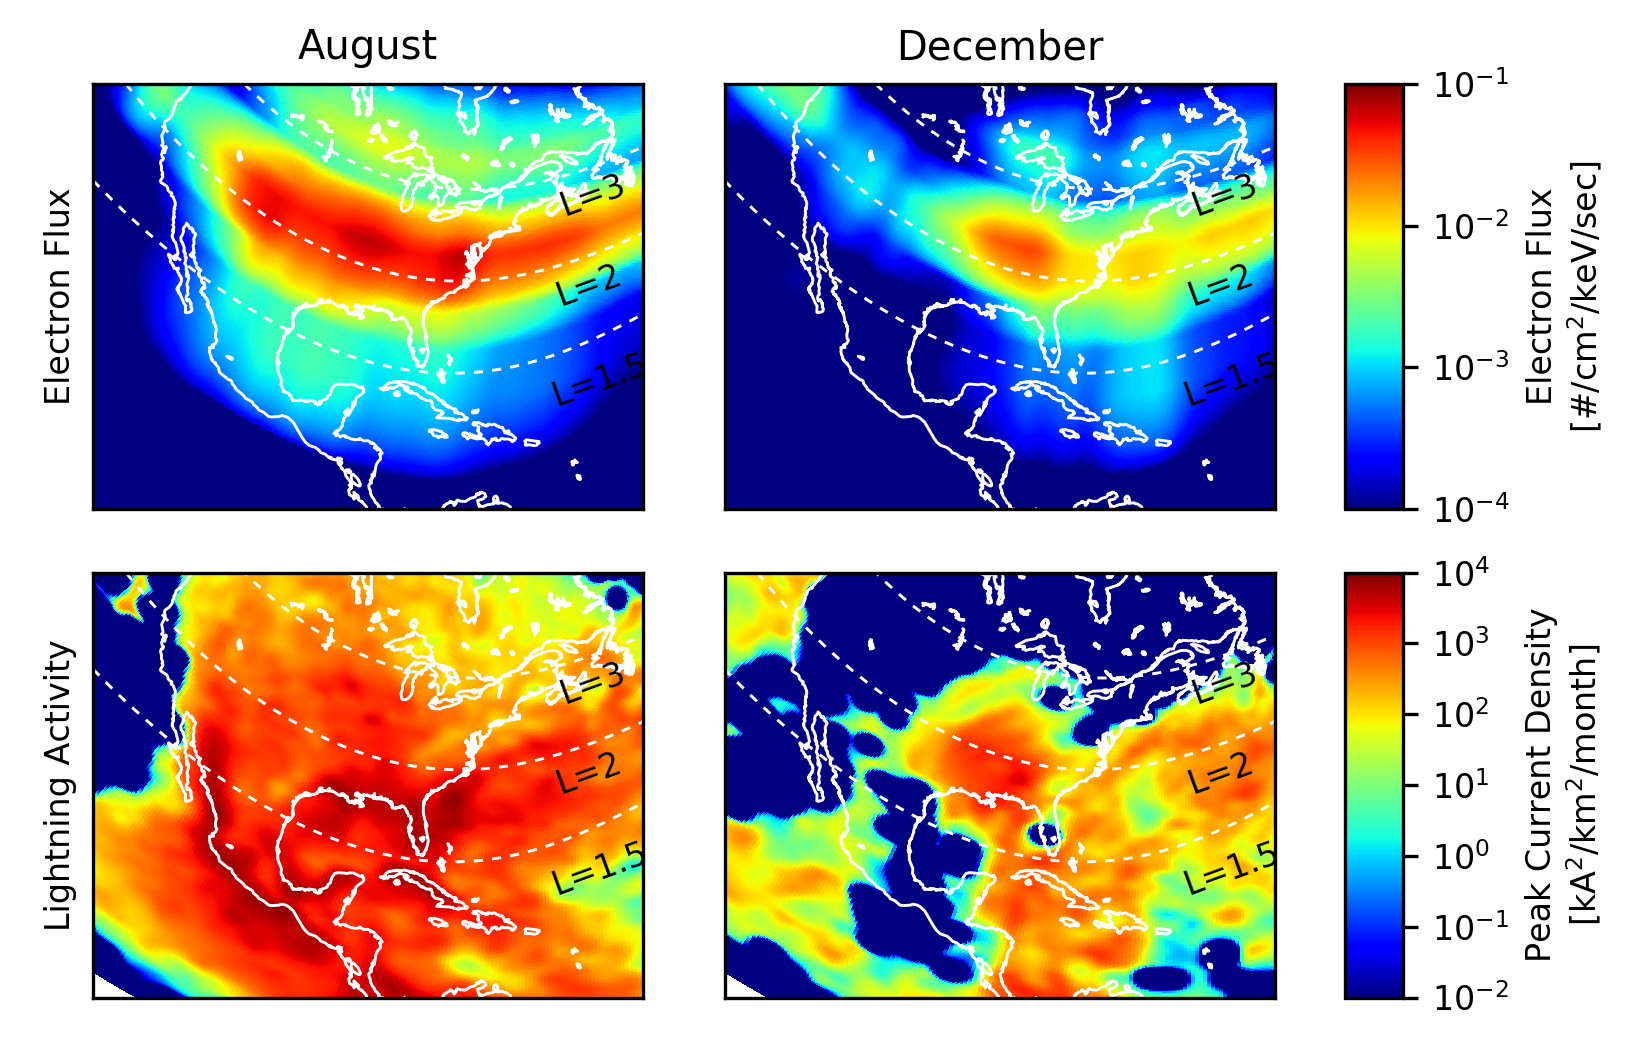
\includegraphics{figures/Gemelos_comparison.png}
\caption[Precipitation at 123 keV over the continental United States, for summer and winter]{Average precipitation at 123 keV over the continental United States, for summer (August) and winter (December). The bottom plots show the corresponding northern-hemisphere lightning as measured by GLD360.}
\label{fig:gemelos_comparison}
\end{center}
\end{figure}

Figure \ref{fig:Meredith_comparison} compares our estimated electron lifetimes to those reported by \cite{Meredith2007}. \citeauthor{Meredith2007} estimates electron lifetimes using a database of magnetosphere VLF wave measurements from the CRRES spacecraft; they then compute pitch angle scattering using the PADIE code, for a variety of assumed wave conditions. \citeauthor{Meredith2007} concludes that pitch angle scattering due to magnetospherically-reflecting whistlers (e.g., LEP) is of little relevance to relativistic electron lifetimes. However, \citeauthor{Meredith2007} uses an incoherent, quasilinear diffusion model, and therefore may not capture the effects of resonant pitch-angle scattering.

Our work is somewhat consistent, in that within the specified energy band, both works show lifetimes much greater than expected, suggesting that LEP is not a dominant loss mechanism. However, our model does show shorter lifetimes at lower L-shells. Additionally, \citeauthor{Meredith2007} does not examine lifetimes of lower energy electrons, for which our model shows the strongest losses. 
\begin{figure}[]
\begin{center}
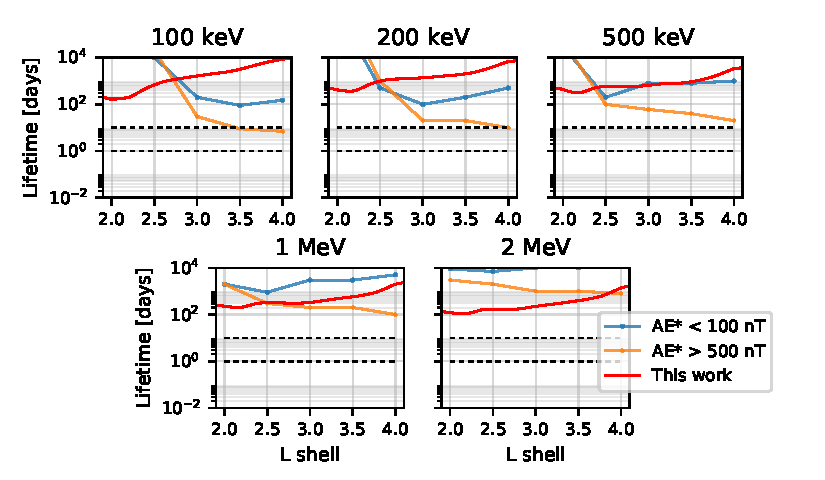
\includegraphics{figures/Meredith_comparison_thesis.pdf}
\caption[Electron lifetime estimates compared against \cite{Meredith2007}]{Comparison of estimated electron lifetimes with those of \cite{Meredith2007}. Red lines show our results; blue lines show \cite{Meredith2007} estimates for quiet geomagnetic conditions; and orange for active geomagnetic conditions. Dashed black lines indicate the approximate measured lifetime of electrons (1 to 10 days).}
\label{fig:Meredith_comparison}
\end{center}
\end{figure}

